\documentclass[a4paper, 11pt]{report}
\setcounter{tocdepth}{3}
\setcounter{secnumdepth}{3}
\usepackage{a4}

\usepackage{pdfpages}
\usepackage[utf8]{inputenc}
\usepackage{dsfont}
\usepackage{amsmath}
\usepackage{graphicx}
\usepackage{here}
\usepackage[section]{placeins}
\usepackage[ngerman]{babel}
\usepackage[font=small,labelfont=bf,margin=\parindent,tableposition=top]{caption}
\usepackage{subcaption}
\usepackage{setspace}

\usepackage[colorlinks, pdfpagelabels, pdfstartview = FitH, bookmarksopen = true, bookmarksnumbered = true, linkcolor = black, plainpages = false, hypertexnames = false, citecolor = black, urlcolor = blue] {hyperref}
\parindent 0pt


\title{Dokumentation der Projektarbeit - Carrera Bahn}
\author{Florian Weber - 44907}
\date{\today}

\begin{document}
\maketitle	%Deckblatt

\begin{spacing}{0.9}
\tableofcontents 	%Inhaltsverzeichnis

\listoffigures		%Bildverzeichnis
\listoftables
\end{spacing}
\newpage

\chapter{Vorwort}%TITEL ÜBERARBEITEN
	\begin{figure}[b]
	\centering
	\includegraphics[width=0.95\textwidth]{rec/Carrerabahnroh.png}
	\caption[Überblick über die Carrera Bahn]{Überblick über die Carrera Bahn mit den Photovoltaik Modulen, der Steuerung mit dem Human Machine Interface (HMI), sowie der Bahn mit den markierten Sensorpositionen.}
	\label{img:carrerakomplett}
	\end{figure}
Die Carrera Bahn ist in Abbildung \ref{img:carrerakomplett} dargestellt. Sie ermöglicht es, zwei Autos gegeneinander antreten zu lassen. Dabei kann bei jedem Auto gewählt werden, ob es automatisch fährt oder durch einen Nutzer manuell gesteuert wird. Die Energieversorgung der jeweiligen Bahn kann unabhängig davon gewählt werden. Es ist dadurch zum Beispiel möglich, als Studierender ein Auto mit Netzstrom manuell, gegen ein automatisch fahrendes Auto, welches mit Solarstrom betrieben wird, zu steuern.
 Dies soll die Chancengleichheit der zwei Energieversorgungen demonstrieren. %

\section{Zustand der Carrera Bahn vor der Projektarbeit}\label{sec:before}
Zu Beginn des Projekts ist die Carrera Bahn auf dem Stand, dass die Fahrzeuge schon konventionell sowie automatisiert betrieben werden können. Außerdem ist die Rundenzeitmessung und deren Visualisierung bereits realisiert. Bei der Energieversorgung kann zwischen Solarstrom und Netzversorgung gewählt werden.
Die Solarstromversorgung wird pro Bahn durch 2 Solarpanels und einem Tiefsetzsteller mit konstantem Dutycycle hergestellt, die Netzstromversorgung mit einem 15V Schaltnetzteil.

Die manuelle Steuerung der Fahrzeuge durch den Nutzer ist realisiert, indem die klassischen Carrera Handregler, als variablen Vorwiderstand zu den Fahrzeugen eingesetzt werden. 
Im automatisierten Modus ist es möglich, mit je einem 5W Potentiometer, die Geschwindigkeit des langsamen Streckenabschnittes einzustellen. In dem schnellen Steckenabschnitt, dem Looping, überbrückt ein Relais diesen Potentiometer und es liegt die volle Betriebsspannung der jeweiligen Energieversorgung am Auto an.
\newpage
\section{Probleme der vorhandenen Carrera Bahn und Zielsetzung zur Projektarbeit}\label{sec:ziel}
Der zuvor erwähnte Aufbau der vorhandenen Anlage vor der Projektarbeit weist einige Probleme auf:
\begin{enumerate}
	\item Solarstromversorgung und Netzversorgung sind nicht chancengleich ausgeführt. (Die Netzversorgung stellt eine stabilisierte Spannungsquelle dar, die Solarstromversorgung eine unstabilisierte Quelle.)
	\item Temperaturdrift des Widerstands des Potentiometers um den Arbeitspunkt im automatisierten Modus.
	\item Framerate der Visualisierung ist zu gering, sodass diese immer die selbe Zahlensequenz nach dem Komma anzeigt.
	\item Manchmal wird durch einen Aliasingeffekt das Überfahren eines Sensors in der Bahn nicht erkannt und die Geschwindigkeit wird nicht umgeschalten. (Echtzeitfähigkeit des Betriebssystems Raspian ist nicht gegeben)
\end{enumerate}
Die oben genannten Probleme sollen im Rahmen der Projektarbeit durch ein neues Steuer-/Regelkonzept, sowie einen Mikrocontroller mit echtzeitfähiger Software gelöst werden.


\chapter{Funktion - Hardware}
	Im Folgenden wird der grundlegende Aufbau der Carrera Bahn nach Abschluss der Projektarbeit erklärt.

	Diese Beschreibung ist immer nur für Bahn-A, da die
	Bahn-B analog dazu funktioniert. Dazu wird immer wieder auf die Abbildung \ref{img:signalfluss}, sowie auf die \\Abbildung
	\ref{img:carrerakomplett} Bezug genommen.\\
	Die Sensoren in den Schienen teilen die Bahn in 3 Streckenabschnitte auf:
	\begin{enumerate}
		\item Startlinie $\rightarrow$ Vor dem Looping
		\item Vor dem Looping $\rightarrow$ Nach dem Looping
		\item Nach dem Looping $\rightarrow$ Startlinie
	\end{enumerate}
	Auf Abschnitt 1 und Abschnitt 3 wird im automatisierten Modus die mittlere Geschwindigkeit des Autos geregelt.
	Im Looping (Streckenbschnitt 2) wird die Spannung auf einen konstanten Wert geregelt.
	Die Grenze dafür ist durch die Position der Sensoren festgelegt und somit nicht variabel.
Wie in Abbildung \ref{img:energiefluss} zu sehen ist, ist der Tiefsetzsteller (TSS) immer zwischen die Energiequelle und das Auto geschaltet. Somit ist es möglich die Bahnspannung zu steuern. 
	\begin{figure}[ht]
		\centering
		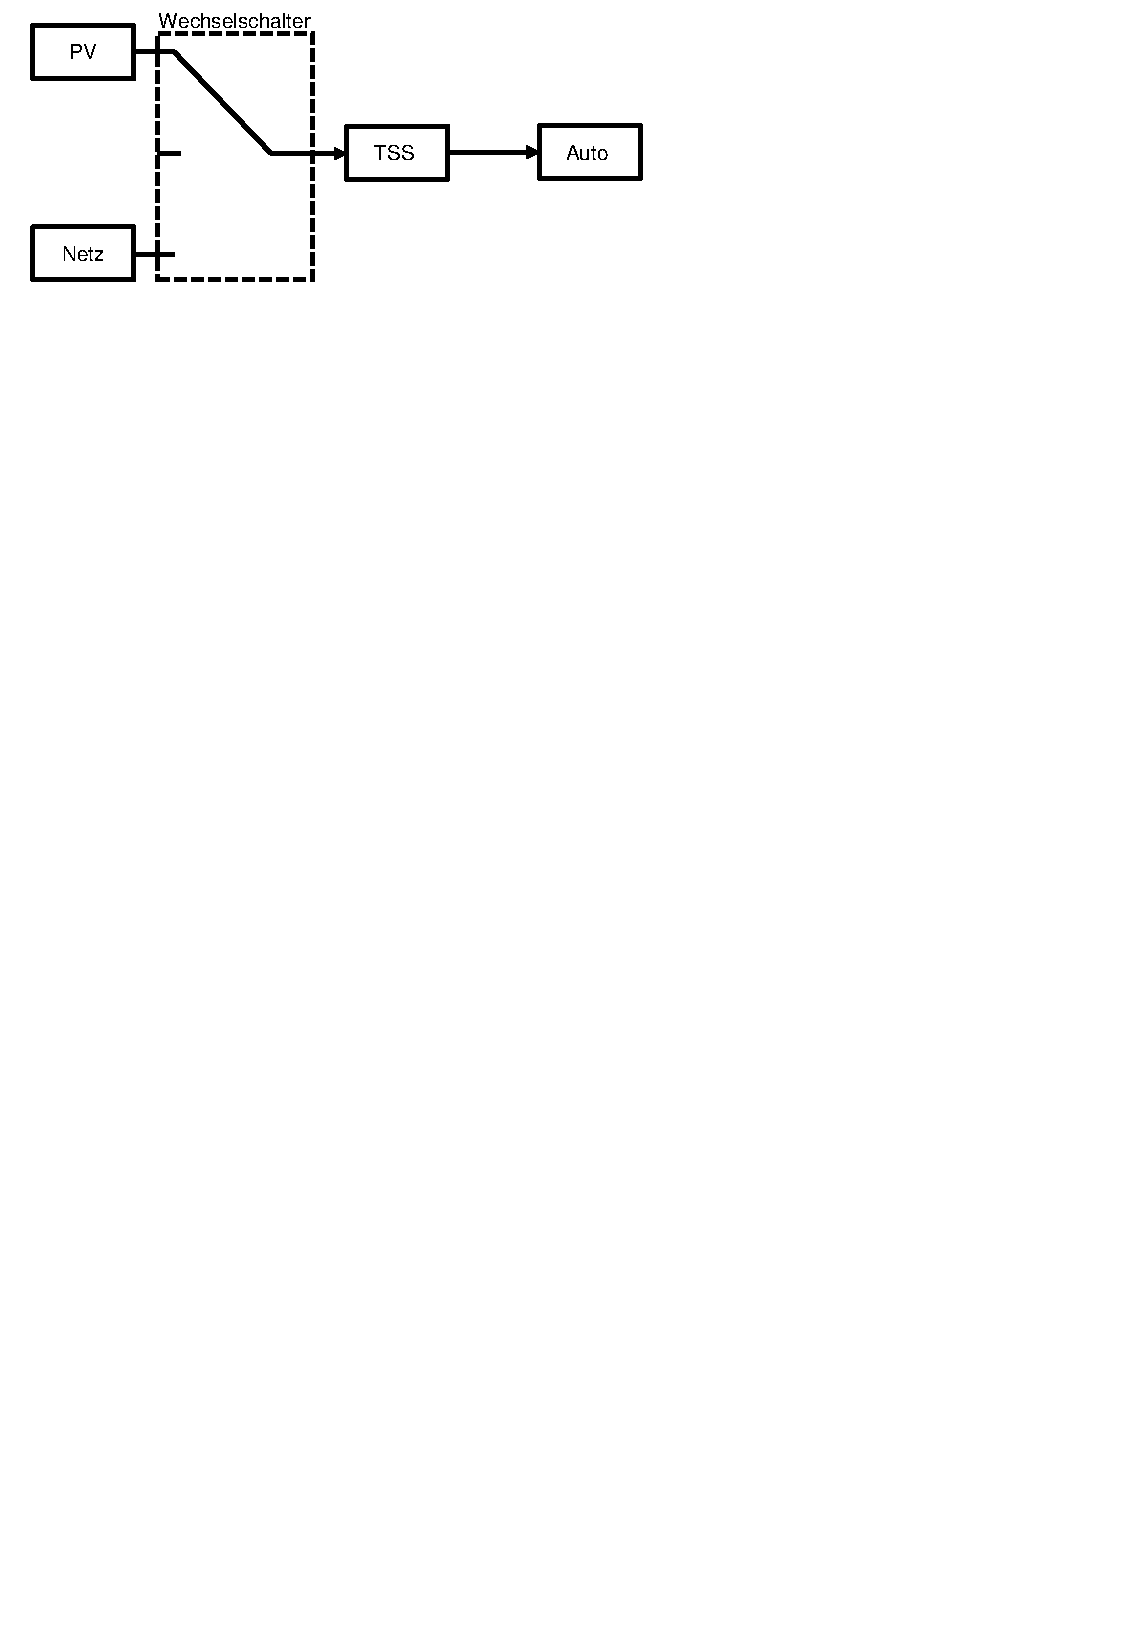
\includegraphics[width=0.85\textwidth]{rec/energiefluss.pdf}
		\caption[Energiefluss einer Bahn]{Energiefluss einer Bahn.\\Durch einen Wechselschalter kann der Nutzer zwischen den zwei Energieversorgungen 
			Photovoltaik (PV) und Netz wählen, oder die Versorgung komplett ausschalten. 
			Der Tiefsetzsteller (TSS) ist dabei immer zwischen Energiequelle und dem Auto auf der Bahn geschaltet.}
		\label{img:energiefluss}
	\end{figure}
	\begin{figure}[ht]
		\centering
		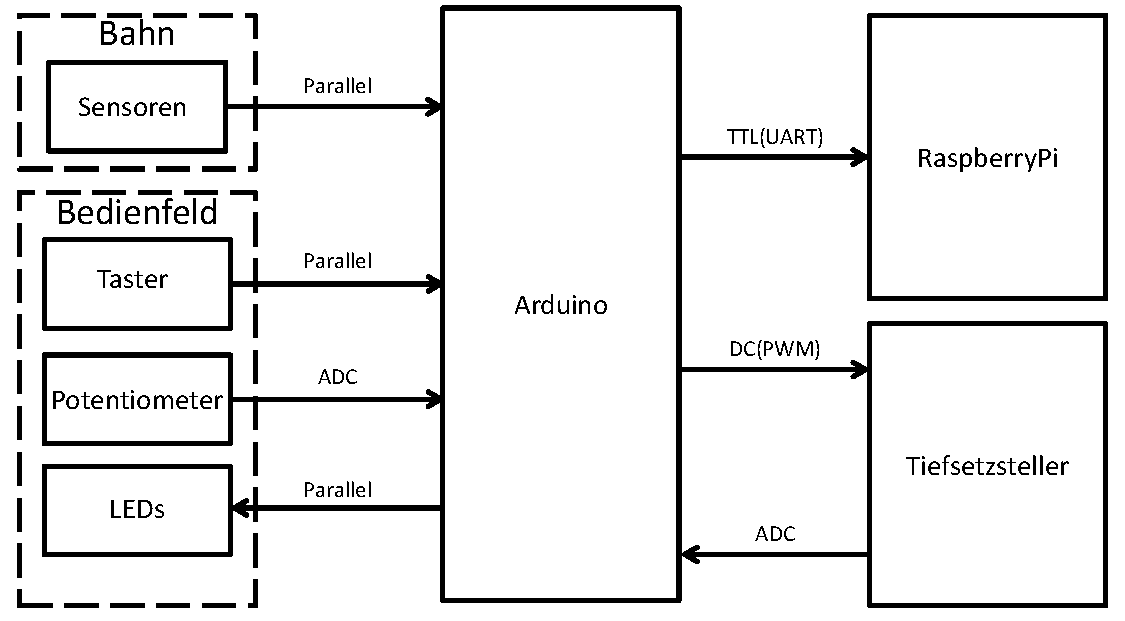
\includegraphics[width=0.85\textwidth]{rec/signalfluss.pdf}
		\caption[Signalflussbild der Steuerung]{Signalflussbild der Steuerung. \\Der Arduino liest Signale von Sensoren, sowie Tastern parallel aus und misst die Ausgangsspannung der Tiefsetzsteller (TSS) und Handregler. Auf Grundlage dieser Daten generiert der Arduino die PWM Signale für die TSS und leitet die Sensordaten per Universal Asynchronous Receiver Transmitter (UART), an den RaspberryPi zur Rundenzeitmessung weiter.}
		\label{img:signalfluss}
	\end{figure}
	
	In Abbildung \ref{img:signalfluss} ist eine Übersicht über den Signalfluss der Carrera Bahn dargestellt.
	Auf der Bahn stellt der Arduino das zentrale Element dar.
	Dieser liest die Sensoren in den Schienen, sowie die Taster des Human Machine Interfaces (HMI) parallel ein und gibt die Signale der LEDs, welche den aktuellen Zustand des jeweils aktiven Modus signalisieren, parallel aus.
	Die analogen Größen (Ausgangsspannung TSS, Spannung über Strommessshunt TSS, Ausgangsspannung Spannungsteiler Handregler) sind an den Analog-Digital-Wandler (ADC) des Arduinos angeschlossen.
	Der Arduino generiert außerdem die zwei PWM Signale, die von den Tiefsetzstellern benötigt werden, über einen 8-bit Hardwaretimer.
	Dies ist genauer in Abschnitt \ref{subsec:PWM} beschrieben.
	Um eine Visualisierung zu realisieren ist ein RaspberryPi per Universal Asynchronous Receiver Transmitter (UART) seriell angebunden. Wie die anderen Kommunikationsverbindungen, ist auch diese Verbindung nur unidirektional ausgeführt.
	Die genaue Implementierung der Schnittstellen ist in den jeweiligen Kapiteln genauer beschrieben.

	\section{Sensoren}
		Wie in Abbildung \ref{img:carrerakomplett} zu sehen ist, gibt es pro Bahn 3 Sensoren. Diese sind als Gabellichtschranken ausgeführt. Sensor 0 befindet sich am Start von Bahn A, Sensor 1 vor dem Looping und Sensor 2 nach dem Looping.\\


		Sensor 0 wird ausschließlich zur Zeitmessung genutzt.
		Sensor 1 wird genutzt um ein Signal zu generieren, so dass die Steuerung das Auto im Automatik-Modus für den Looping beschleunigen kann.
		Das Signal von Sensor 2 wird schließlich genutzt um nach dem Looping wieder die langsame Geschwindigkeit zu triggern.\\
		Sensor 3 bis 5 stellen die selben Signale, analog zu Bahn A, von Bahn B bereit.

		Im manuellen Modus dienen die Sensoren nur zur Zeitmessung für die Visualisierung.

		Da die Flanke eines Sensors nur sehr kurz ist, lässt sich diese nicht per Polling ohne Aliasing Effekte digitalisieren. Stattdessen werden die Signale der Bahnsensoren durch Hardware Pin Change Interrupts (PCINT) des Arduino digitalisiert.
		Die Funktionsweise dieser PCINTs ist genauer im Abschnitt \ref{subsubsec:PCINT} erklärt
	\section{Human Machine Interface}
		\begin{figure}[b]
			\centering
			\includegraphics[width=0.95\textwidth]{rec/hid.png}
			\caption{HMI mit Arduino, RaspberryPi und TSS}

			\label{img:hid}
		\end{figure}
		Wie in Abbildung \ref{img:hid} dargestellt, besteht das Human Machine Interface (HMI) aus drei Wechseltastern mit Mittelstellung, sowie zwei Wechselschaltern mit Mittelstellung.

		Der Wechselschalter (\glqq Wechselschalter 0\grqq{} für Bahn A und \glqq Wechselschalter 1\grqq{} für Bahn B ) ist zum Auswählen der Energieversorgung der jeweiligen Bahn. In der oberen Stellung wird die Bahn mit Netzenergie versorgt, in der unteren Stellung mit Solarenergie.
Ist einer dieser Wechselschalter in Mittelstellung, wird die Bahn nicht versorgt und das entsprechende Auto steht, unabhängig des gewählten Modus.\\
		Über die Wechseltaster 0 beziehungsweise Wechseltaster 2 lässt sich der Modus der zugehörigen Bahn auswählen. Dies erfolgt indem einer der Taster oben beziehungsweise unten betätigt wird.  Der aktuell ausgewählte Modus wird durch die LEDs über beziehungsweise unter den Tastern signalisiert. Das LED oben signalisiert dabei den manuellen Modus, indem das Auto durch den Handregler gesteuert wird und ein LED unten, den Modus indem das Auto selbstständig fährt.\\
Mit Wechseltaster 1  lassen sich die Integratoren der Regler, der Bahngeschwindigkeit (Abbildung \ref{fig:Tcontrol}), welche ausschließlich im automatisierten Modus aktiv sind, auf ihren Startwert zurücksetzten. Dabei setzt ein oberer Tastendruck den Regler von Bahn A und ein unterer den Regler von Bahn B zurück. Diese Regler sind genauer in Abschnitt \ref{subsec:control} beschrieben.
Global existiert noch ein weiterer Taster um die Visualisierung (Rundenzeitmessung) zurückzusetzen. Dieser ist in Abblidung \ref{img:hid} mit \glqq Reset Visualisierung\grqq{} beschriftet und befindet sich zwischen den zwei Tiefsetzstellern oben links.
	\section{Arduino}
		Beim Arduino handelt es sich um einen Arduino Mega 2560 ADK.\\
		Dieser ist mit einem ATmega2560 der Firma Microchip bestückt.
		Der ATmega2560 ist perfekt für die Anwendung geeignet, da er einen Analog-Digital-Wandler (ADC) zur Messung analoger Größen, Hardwaretimer mit PWM Funktionalität, sowie  vier UARTs zur Kommunikation besitzt.
Der Arduino kommt zum Einsatz, da er die Pins des Mikrocontrollers auf Buchsenleisten führt. So ist es unter anderem möglich, ohne größeren Aufwand, Drähte an die Pads der Buchsenleisten anzulöten, oder zu Demonstrationszwecken ein Oszilloskop anzuschließen. Außerdem enthält ein Arduino bereits alle zum Betrieb notwendigen Bauteile für den Mikrocontroller.
Dies sind zum Beispiel die Abblockkondensatoren an der Versorgungsspannung oder der Glättungskondensator an der Referenzspannung des ADCs.
Des Weiteren enthält der Arduino einen USB-Seriell Wandler, der genutzt werden kann, um sich Daten parallel zum Prozess an ein Terminal auszugeben.
Dies ist zum Beispiel sehr hilfreich, um das Programm zu debuggen, oder die Regelparameter einzustellen.
Der Mikrocontroller ist mit 16MHz getaktet und wird direkt mit 5V aus dem Steckernetzteil des RaspberryPi versorgt.
	\section{RaspberryPi}
		Die Visualisierung ist durch ein RaspberryPi Model 3 B+ realisiert. Dieser empfängt per UART die codierten Signale der Sensoren, sowie des Tasters \glqq Reset Visualisierung\grqq{} (siehe Abbildung \ref{img:hid}).
		Die Visualisierung ist zu Beginn der Projektarbeit bereits vorhanden und in Form eines Python Skripts implementiert.
	\section{Tiefsetzsteller}
		Die Tiefsetzsteller (TSS) fungieren als Stellglieder der Spannungsregelungen der Bahnen.
		Dabei sind die Bahnen jeweils direkt an die Ausgänge der beiden TSS angeschlossen.
	  Der Arduino generiert die zwei PWM Signale für die TSS.
		Die Ausgangsspannung der TSS wird vom Arduino gemessen und durch den in Abschnitt \ref{subsubsec:Ucontrol} beschriebenen Regelkreis auf ihre aktuellen Sollwerte geregelt.
		Die maximale Ausgangsspannung eines TSS ist lediglich durch die Leerlaufspannung eines PV-Strangs (21V\textsubscript{max})
		nach oben hin begrenzt.
		Da diese größer sein kann als die Referenzspannung des ADC (V\textsubscript{ref}=V\textsubscript{CC} = 5V), wird sie über einen Spannungsteiler auf 5V\textsubscript{max} angepasst und auf einen Kanal des Analog-Digital-Wandlers des Mikrocontrollers geführt. Dies bewirkt die größtmögliche Aussteuerung des ADC ohne das dieser übersteuert wird.
		Des Weiteren ist über ein Shunt eine Strommessung realisiert.
		Dieser Stromwert liegt zwar im Arduino digital vor, wird allerdings nicht weiter
		verarbeitet und ist lediglich für weiterführende Projekte gedacht.
\chapter{Software}
	\section{RaspberryPi}\label{sec:SoftPi}
		Bei der Software, die auf dem RaspberryPi ausgeführt wird, handelt es sich um ein Python Skript.
		Das Script bekommt die Signale der Sensoren, sowie des Tasters \glqq Reset Visualisierung \grqq, über die serielle Schnittstelle \glqq ttyAMA0 \grqq, 
		gesendet und führt eine Rundenzeitmessung je Bahn durch.
		Diese Zeitmessung wird auf dem Bildschirm angezeigt.
		Zum Rendern der Schriften sowie dem Hintergrundbild, ist die Open Source Bibliothek \glqq PyGame\grqq{} in Verwendung.
		Das Bild ist separiert in einen Hintergrund und einem Block der den dynamischen Inhalt der Rundenzeitmessung enthält.
		Um die Framerate entgegen der Version aus einer vorherigen Arbeit zu steigern, wird lediglich der dynamische Inhalt framweise neu gerendert.
	\section{Arduino}
		Die Software des Arduinos ist nicht in der Arduino Entwicklungsumgebung geschrieben, da dies einen direkten Zugriff auf die Hardware erschwert und der Programmablauf bereits vorgegeben wäre.
		Stattdessen ist die Software in der integrierten Entwicklungsumgebung (IDE) \glqq Atmelstudio 7.0\grqq{} entwickelt.
		Der Bootloader des Arduino ist entfernt.
		Das ermöglicht nun einen direkten Zugriff auf die Prozessorregister und damit Konfiguration der einzelnen Komponenten des Mikrocontrollers auf dem Arduino.
		Dias ist notwendig, um das Timing des Controllers exakt zu steuern und ist effizienter als für alle Hardwarekomponenten eine Bibliothek zu nutzen wie es die Arduino Entwicklungsumgebung vorsehen würde.
\newpage
		\subsection{Interrupts}
		\begin{figure}[ht]
			\centering
			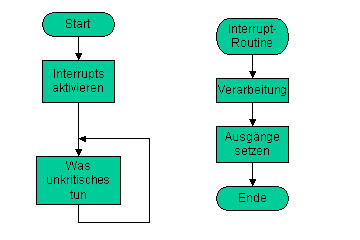
\includegraphics[width=0.8\textwidth]{rec/Interrupt_Programme.png}
			\caption[Interruptgesteuerter Programmablauf]{Interruptgesteuerter Programmablauf \hyperref[src:scout1]{[scout1]}}
			\label{InterruptgesteuerterProgrammablauf}
		\end{figure}
Der Programmablauf ist interruptgesteuert und folgt damit dem Modell in Abbildung \ref{InterruptgesteuerterProgrammablauf}.
			Dies hat den Vorteil, dass das Timing nicht mehr von der Länge der MainLoop abhängt und Vorgänge wie zum  Beispiel der Regelalgorithmus immer mit der selben Frequenz ausgeführt werden.
			In der Mainloop des Programms werden zeitunkritische Aufgaben erledigt, wie die LEDs der HMI zu aktualisieren.
			Interruptquellen des Programms sind:
			\begin{itemize}
				\item Timer  (Abschnitt \ref{subsubsec:Timer})
				\begin{itemize}
					\item[1.] Timer1, Compareregister B match
					\item[2.] Timer3, Compareregister A match
					\item[3.] Timer4, Compareregister A match
				\end{itemize}
				\item Pin Change Interrupts (Abschnitt \ref{subsubsec:PCINT})
				\begin{itemize}
					\item[4.] PCINT0\underline{ }vect
					\item[5.] PCINT1\underline{ }vect
					\item[6.] PCINT2\underline{ }vect
				\end{itemize}
				\item Analog Digital Converter
				\begin{itemize}
					\item[7.] ADC\underline{ }vect  (Abschnitt \ref{subsubsec:ADCINT})
				\end{itemize}

			\end{itemize}
			\subsubsection{Timer}\label{subsubsec:Timer}
			Für die Funktion der Steuerung werden viele Timer benötigt.\\
			Da im Mikrocontroller allerdings nur begrenzt Hardwaretimer zur Verfügung stehen, ist deren Funktionalität in einem Softwaretimer nachgebildet.
			Dieser bezieht seinen Takt von dem  Hardwaretimer \glqq Timer4\grqq.
			Die Verwendung der Hard- sowie Softwaretimer kann der Tabelle \ref{tab:belegungTimer} entnommen werden.
				\begin{table}[ht]
					\caption{Belegung der Hard- sowie Softwaretimer}
					\begin{tabular}{|l|l|l|}
						\hline
						\textbf{Timer} & \textbf{Funktion}\\
						\hline
						\hline
						 & \\
						Hardwaretimer &\\
						\hline
						\hline
						Timer0 & Generierung der 2 PWM Kanäle für die Tiefsetzsteller\\
						\hline
						Timer1 & Auslösen der Analog Digital Wandlung\\
						\hline
						Timer2 & Ohne Verwendung\\
						\hline
						Timer3 & Trigger für Spannungsregelung\\
						\hline
						Timer4 & Trigger für Softwaretimer\\
						\hline
						\hline
						 & \\
						Softwaretimer &\\
						\hline
						\hline
						0..1 & Zeitmessung Abschnitt 3 (Nach dem Looping $\rightarrow$ Startlinie)\\
						\hline
						2..7 & Entprellen der Bahnsensoren\\
						\hline
						8..14 & Entprellen der HID Taster\\
						\hline
						15..16 & Ohne Verwendung\\
						\hline
						17 & Trigger für Zeitmessung Resettaster Visualisierung (langer Tastendruck)\\
						\hline
					\end{tabular}
					
					\label{tab:belegungTimer}
				\end{table}
			\subsubsection {Pin Change Interrupt}\label{subsubsec:PCINT}
			
			Wenn ein Auto auf beispielsweise Sensor 0 (Bahn A, an der Startlinie) fährt, wird der Pegel kurze Zeit \emph{Low} und nach Verlassen des Sensors wieder \emph{High}.\\ Sensor 0 ist nach Tabelle \ref{tab:belegungpcint} an PCINT16 angeschlossen. 
			Aus dem Datenblatt des Mikrocontrollers (ATmega2560) geht hervor, dass für die Pin Change Interrupts drei Interruptvektoren vorgesehen sind. 
			Dabei besteht eine Zuordnung von jeweils immer acht PCINT Pins an einen Interruptvektor. 
			Diese Zuordnung beginnt bei dem Pin PCINT0 und PCINT0\underline{}vect. 
			Durch das Überfahren des Autos über den Sensor wird also das letzte Pin Change Interrupt, PCINT2\underline{ }vect, zweimal ausgelöst. 
			In der Interrupt Service Routine (ISR) muss nun unterschieden werden durch welchen Pin das Interrupt ausgelöst wurde.
			Die Lösung dieses Problems ist gegeben, indem der Signalpegel der PCINT Pins in der letzten ISR gesichert werden. Nun wird das aktuelle Eingangsbyte des Ports mit dem zuvor gespeicherten bitweise exklusiv-oder verknüpft.
			Ist das Ergebnis der Verknüpfung nicht \glqq 0\grqq, entspricht die Stelle der logischen \glqq 1\grqq im Byte, der Nummer des PCINT Pins gezählt, von dem ersten zugeordneten Interruptpin des Bytes. 
			So ist das Ergebnis der exklusiv-oder Verknüpfung dieses Beispiels mit Sensor 0: $00000001$ da sich das nullte Bit verändert hat.
			In der ISR muss nun weiter, zwischen den zwei Möglichkeiten, unterschieden werden:
				\begin{itemize}
					\item \emph{High$\rightarrow$Low} Übergang
					\item \emph{Low$\rightarrow$High} Übergang
				\end{itemize}
			Hat ein \emph{High$\rightarrow$Low} Übergang stattgefunden, wird ein Event erzeugt und je nach PCINT Pin unterschiedlich behandelt.
			Bei einem \emph{Low$\rightarrow$High} Übergang kann das Ereignis verworfen werden.

			Das Entprellen des Eingangs ist implementiert, indem nach dem Auslösen eines Events, die PCINT Funktion für den zugehörigen Pin deaktiviert wird, sodass dieser das Interrupt nicht mehr auslösen kann. Zusätzlich wird ein Softwaretimer gestartet, der die PCINT Funktion des Pins, nach dessen Ablauf wieder aktiviert. Mit diesem einfachen Prinzip wird sichergestellt, dass das Auto beim Überfahren des Sensors das dementsprechende Event nur einmal triggert.
			Analog zu dem Sensor 0 ist dies für jeden Sensor sowie Taster implementiert. Die Belegung der benutzten Pin Change Interrupts kann Tabelle \ref{tab:belegungpcint} entnommen werden.
			\begin{table}[ht]
				\caption{Belegung der Pin Change Interrupts}
				\begin{tabular}{|l|l|l|}
					\hline
					Zugehörigkeit & Signal & Bezeichnung\\
					\hline
					\hline
					PCINT0\underline{ }vect & PCINT4 & Button: B-Automatik\\
					\hline
											& PCINT5 & Button: B-Manuell\\
					\hline
											& PCINT6 & Button: A-Automatik\\
					\hline
					\hline
					PCINT1\underline{ }vect & PCINT9 & Button: A-Reset\\
					\hline
											& PCINT10 & Button: B-Reset\\
					\hline
					\hline
					PCINT2\underline{ }vect & PCINT16 & Sensor: 0\\
					\hline
											& PCINT17 & Sensor: 1\\
					\hline
											& PCINT18 & Sensor: 2\\
					\hline
											& PCINT19 & Sensor: 3\\
					\hline
											& PCINT20 & Sensor: 4\\
					\hline
											& PCINT21 & Sensor: 5\\
					\hline
											& PCINT22 & Button: Reset/Shutdown Pi\\
					\hline
											& PCINT23 & Button: A-Manuell\\
					\hline
				\end{tabular}
				\label{tab:belegungpcint}
			\end{table}
				\paragraph{Unterschied: Pin Change Interrupt - Polling mit echtzeitfähigem System - Polling ohne echtzeitfähigem System}\mbox{}\\
					Wie in Abbildung \ref{fig:rtPolling} dargestellt, gibt es zwei Möglichkeiten, ein wertdiskretes Signal mit den gültigen Zuständen High oder Low zu digitalisieren.
					Die erste Möglichkeit ist die zyklische Abfrage des Zustands. Dieses Verfahren wird in der Informatik Polling genannt.
					Bei Polling ist zu beachten, dass das Abtasttheorem eingehalten wird. 
					Dieses besagt, es muss mit mindestens der doppelten Frequenz des abzutastenden Signals abgetastet werden, 
					anderenfalls kommt es zu Aliasing und es ist nicht mehr möglich, das abgetastete Signal ohne Informationsverlust zu rekonstruieren.
					Da in einem nicht echtzeitfähigen Betriebssystem, wie zum Beispiel Raspian, nicht garantiert werden kann, 
					dass die Signalabtastung lückenfrei, in äquidistanten Zeitabständen stattfindet,
					ist die Einhaltung des Abtasttheorems und damit das Vermeiden von Aliasingfehlern nicht gesichert.
					Ein solchen Fehler ist in Abbildung \ref{fig:rtPolling} mit der roten Datenreihe dargestellt. Hier ist einem anderen Prozess, 
					innerhalb der zu detektierenden Signalflanke, Rechenzeit zugeteilt worden, sodass die Abtastung des Signals in dieser Zeit ausfällt.
					Genau dieses Verhalten führt zu dem in Abschnitt \ref{sec:before} beschrieben Problem, dass Sensoren nicht zuverlässig detektiert werden.

\newpage
					Eine Alternative zu Polling, stellt ein Abtasten der Signalflanken durch eine Hardwareeinheit wie sie in einem Atmega2560 integriert ist dar.
					Diese Hardwareeinheit tastet nun in den Zeitabständen der Taktversorgung des Mikrocontrollers (in dieser Arbeit: 16MHz) das Signal ab 
					und löst bei jeder Änderung ein Hardwareinterrupt aus. 
					Somit ist garantiert, dass die Flanken sicher erkannt werden. 
					In der vorliegenden Projektarbeit sind deshalb Pin Change Interrupts in Verwendung, zuvor war dies nicht der Fall.  
				\begin{figure}[ht]
					\centering
					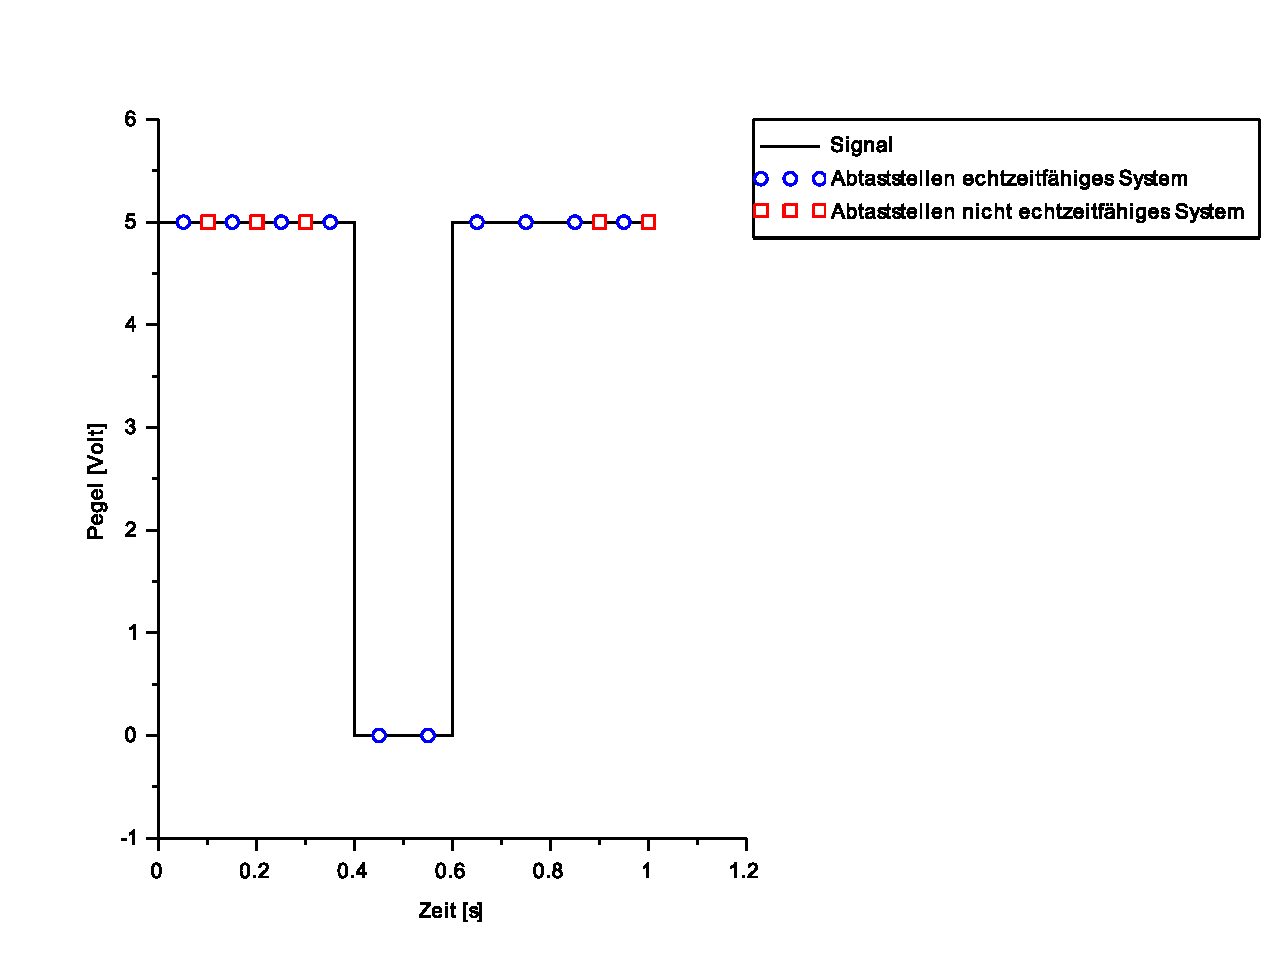
\includegraphics[width=\textwidth]{rec/rtPolling.pdf}
					\caption[Abtastung eines digitalen Signals]{Abtastprozess eines analog vorliegenden wertdiskreten Signals durch Softwarepolling mit echtzeitfähigem System, 
 					Softwarepolling ohne echtzeitfähigem System sowie Hardware Pin Change Interrupts.\\
					Die schwarze Linie stellt ein abzutastendes Beispielsignal dar, wie es zum Beispiel von einem Bahnsensor zu erwarten wäre.
					Die blauen Kreise stellen die Stützstellen einer zyklischen Abtastung eines echtzeitfähigem Systems, 
					mit der vierfachen Abtastrate wie die Grundfrequenz des Signals, 
					dar und die roten Vierecke die Stützstellen bei einem nicht echtzeitfähigen System mit verletztem Abtasttheorem im Bereich der zu detektierenden Flanken.
					 }
				\label{fig:rtPolling}
				\end{figure}
\FloatBarrier
			\subsubsection{Analog Digital Converter Interrupt}\label{subsubsec:ADCINT}
			Zum Betrieb des Zustandsautomats (Abbildung \ref{img:ADCMUX}) welcher den Multiplexer des ADC steuert ist ein Interrupt notwendig, welches ausgelöst wird, wenn der ADC eine Messung abgeschlossen hat. Dieser Automat ist genauer in Abschnitt \ref{subsec:ADC} beschrieben.

			%erklärung an diesem
	\subsection{Regler}\label{subsec:control}
Die Carrera Bahn hat zwei verschiedene Regelkreise. 
Der eine regelt die Bahnspannung (siehe Abschnitt \ref{subsubsec:Ucontrol}) und ist in jedem Modus (manuell oder automatisiert) aktiv. 
Der andere Regelkreis (siehe Abschnitt \ref{subsubsec:Tcontrol}) ist lediglich im automatisierten Modus aktiv und regelt dort die Soll-Spannung auf den langsamen Streckenabschnitten (außerhalb des Loopings).
Zusammen bilden die zwei Regelkreise im automatisierten Modus eine Kaskadenregelung.
		\subsubsection{Bahnspannung}\label{subsubsec:Ucontrol}
			\begin{figure}[ht]
				\centering
				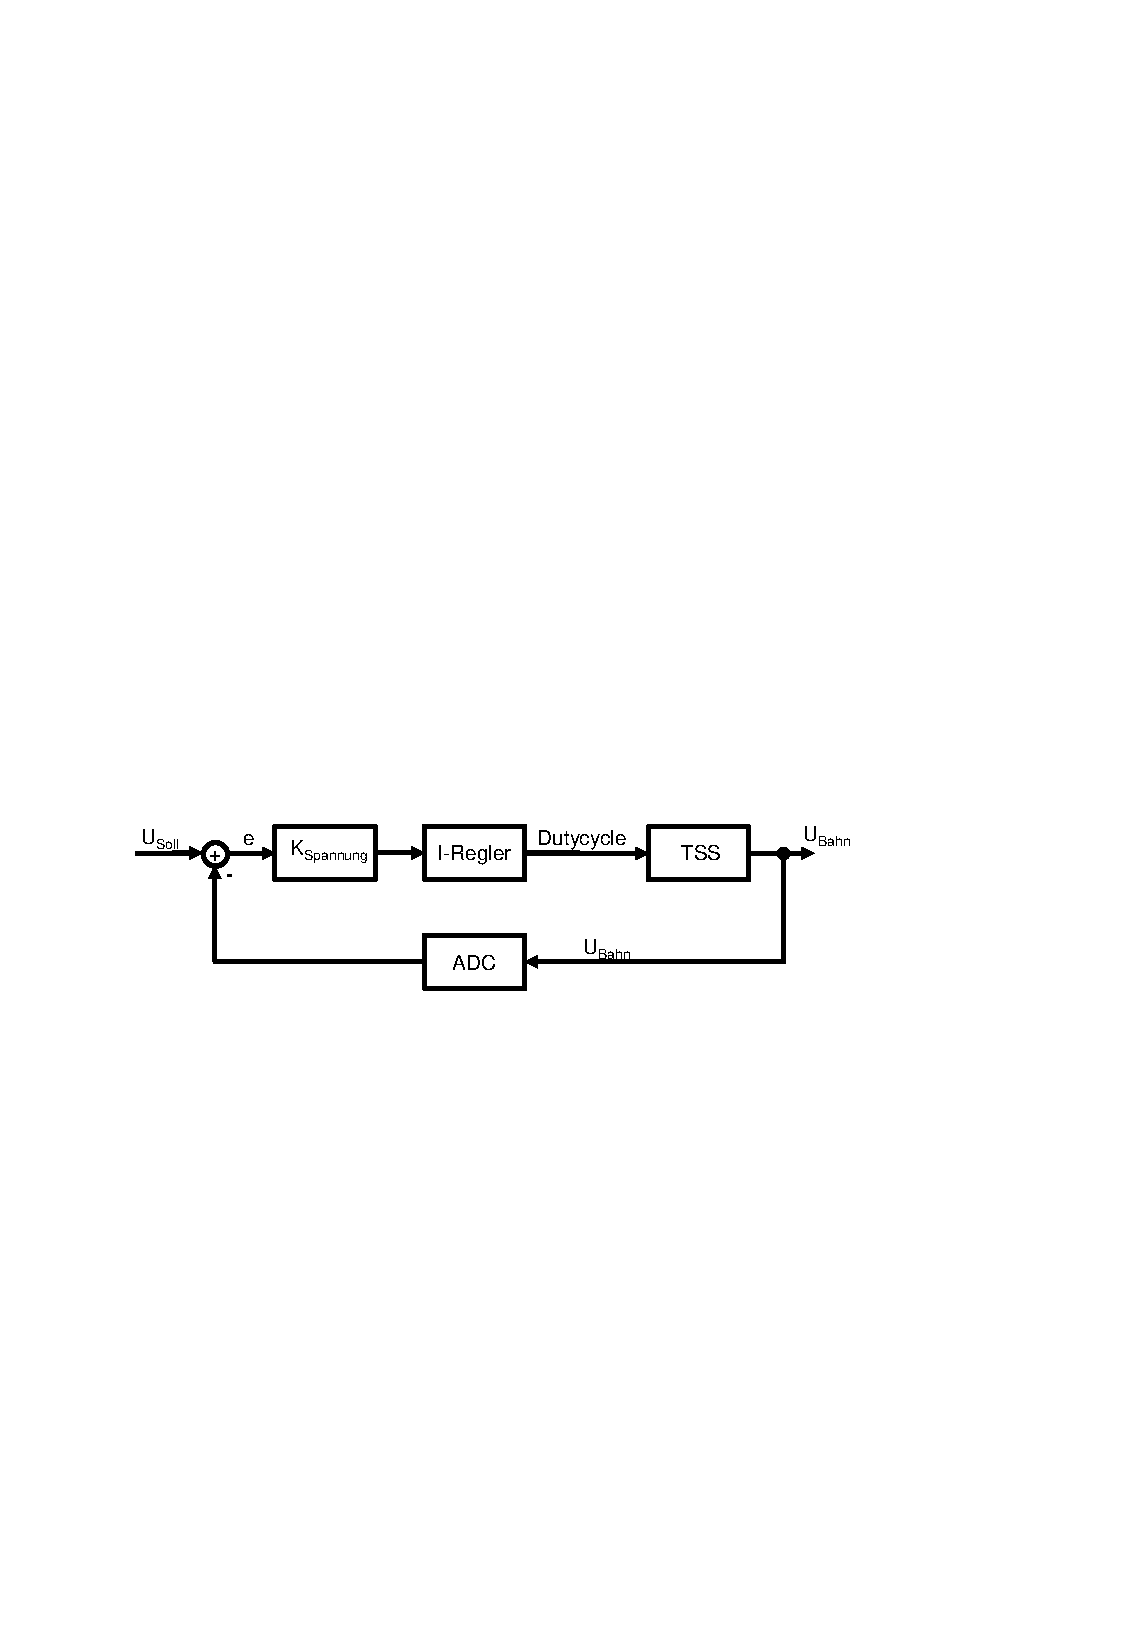
\includegraphics[width=\textwidth]{rec/Ucontrol.pdf}
				\caption[Regelkreis Bahnspannung]{Regelkreis Bahnspannung.\\Die Soll-Spannung wird je nach aktiven Modus der Bahn vorgegeben.
				Die Ist-Spannung der jeweiligen Bahn wird mit dem ADC gemessen und die Regelabweichung errechnet.
				Regelabweichung wird mit dem konstanten Faktor K\textsubscript{Spannung} verstärkt und auf den I-Regler gegeben.
				Dieser erzeugt Den Dutycycle der auf den TSS gegeben wird.
				TSS erzeugt Bahnspannung.}
				\label{fig:Ucontrol}
			\end{figure}
			Um Schwankungen in der Energieversorgung auszugleichen, sowie das Steuern der Bahnspannung zu ermöglichen, 
			ist eine Spannungsregelung nach Abbildung \ref{fig:Ucontrol} implementiert.
			Die Ist-Spannung der jeweiligen Bahn wird zyklisch mittels des ADCs gemessen. Jedes mal wenn ein neuer Wert der Bahnspannung von Bahn-A vorliegt, 
			wird die Funktion  \emph{i\_control\_voltage\_a} (siehe Quellcode)  aufgerufen. Die Funktion kann nun die Regeldifferenz \glqq e\grqq{} bilden und 
			diese mit dem Faktor \glqq K\textsubscript{Spannung}\grqq{} verstärken.
			Der I-Regler (einfacher digitaler Integrator mit der Differenzengleichung $y[k]=y[k-1]+x[k]$) integriert diese verstärkte Regelabweichung auf und 
			generiert damit den Dutycycle für den TSS, bei dem sich dann eine neue Ausgangsspannung (U\textsubscript{Bahn}) entsprechend des neuen Dutycycle einstellt. 
			Diese neue Spannung wird wieder gemessen und die Funktion wird erneut aufgerufen.
			Als Regler ist ein digitaler I-Regler in Verwendung, da Die Strecke (TSS) kein freier Integrator besitzt. 
			Jedoch braucht ein Regelkreis mindestens ein freien Integrator um stationäre Genauigkeit aufzuweisen.
			Zusätzlich zu dem gerade eben beschriebenen Regelalgorithmus, ist die Ausgangsgröße des I-Reglers nach oben (maximal 200/255), 
			sowie unten (minimal 10/255) begrenzt. Dies ist notwendig da der TSS jenseits eines Dutycycle von 200, bei einer weiteren Erhöhung, 
			nicht mehr eine höhere Ausgangsspannung liefert und das Auto sich unter einem Dutycycle von 10 noch nicht bewegt. 
			Diese Grenzen wurden empirisch ermittelt und beziehen sich auf die Quelle mit dem höchsten Innenwiderstand (PV).
		\subsubsection{Bahngeschwindigkeit}\label{subsubsec:Tcontrol}
			\begin{figure}[ht]
				\centering
				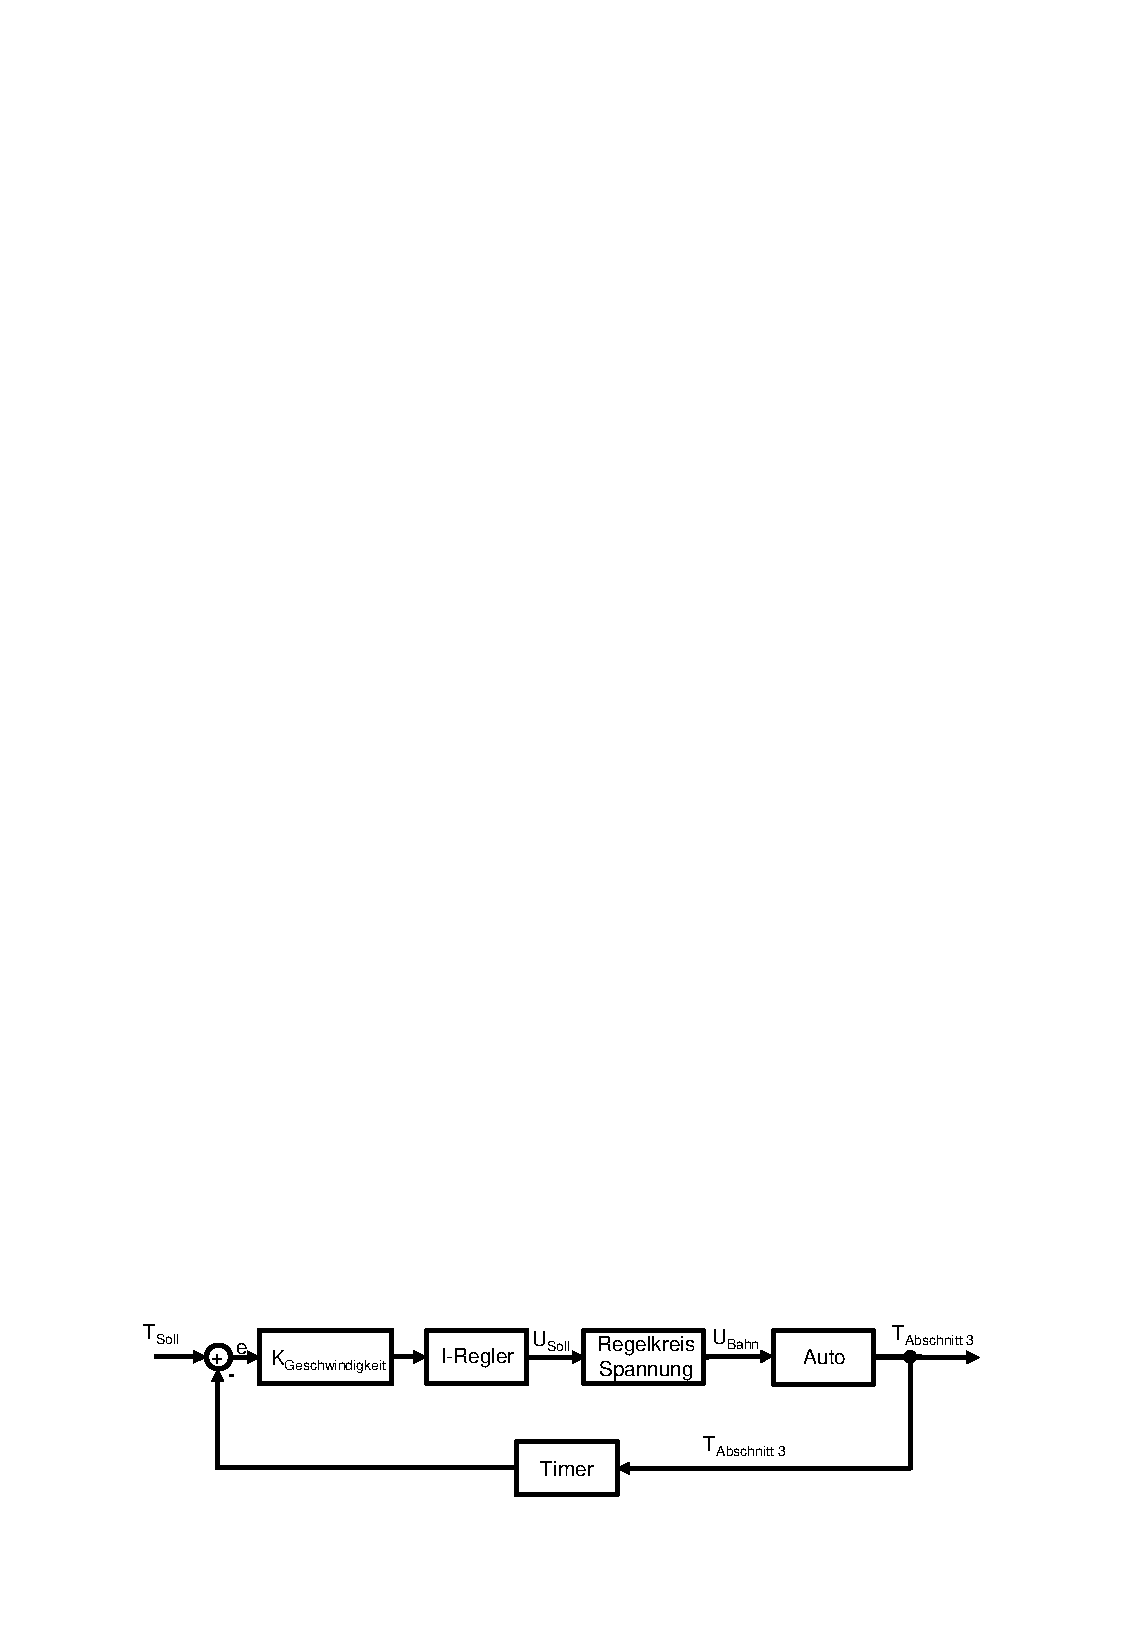
\includegraphics[width=\textwidth]{rec/Tcontrol.pdf}
				\caption[Regelkreis Bahngeschwindigkeit]{Regelkreis Bahngeschwindigkeit.\\
				Die Sollzeit ist als konstanter Parameter vorgegeben.
				Die Zeit in Streckenabschnitt 3 (zwischen dem Ende des Loopings und der Startlinie) wird mit einem Softwaretimer gemessen und mit der Sollzeit verglichen.
				Die resultierende Regelabweichung wird mit dem konstanten Faktor K\textsubscript{Geschwindigkeit} verstärkt und auf den I-Regler gegeben.
				Dieser erzeugt daraus die Soll-Spannung für die jeweilige Bahn und gibt diese an den inneren Regelkreis (Regelkreis Spannung, Abbildung \ref{fig:Ucontrol}) weiter.
				Dieser geneneriert daraus die Ist-Spannung die am Auto anliegt. Daraus ergibt sich eine neue Zeit für den Streckenabschnitt 3.}
				\label{fig:Tcontrol}
			\end{figure}
			Da die Carrera Bahn mit verschiedenen Fahrzeugen betrieben werden kann und somit die Modellparameter nicht konstant sind (zum Beispiel Reibungsverluste im Fahrzeug, allgemein Motor), ist es notwendig die Soll-Spannung im automatisierten Modus auf den langsamen Streckenabschnitten anzupassen. Hierzu ist ein Regler nach Abbildung \ref{fig:Tcontrol} implementiert. Dabei wird die Zeit gemessen, welche das Auto benötigt, um die Strecke zwischen dem Sensor nach dem Looping bis zum Sensor an der Startlinie zu fahren.
Für diese Zeit ist im Arduino eine konstante Soll-Zeit hinterlegt. Jedes mal wenn ein neuer Messwert für die Zeit auf diesem Streckenabschnitt vorliegt, wird die Funktion 
\emph{i\_control\_railspeed\_a}  (siehe Quellcode)  aufgerufen und darin die  Regeldifferenz \glqq e\grqq{} bilden. Analog zu dem Regelkreis in Abschnitt \ref{subsubsec:Ucontrol}, wird auch hier die Regeldifferenz gebildet und mit dem Faktor K\textsubscript{Geschwindigkeit} skaliert. Als Regler kommt ein I-Regler wie in Abschnitt \ref{subsubsec:Ucontrol} zum Einsatz. Die so erzeugte Stellgröße U\textsubscript{Soll} wird nun auf das Stellglied (innerer Regelkreis Bahnspannung aus Abschnitt \ref{subsubsec:Ucontrol}) gegeben und es ergibt sich durch eine neue Bahnspannung auch eine neue Zeit für den gemessenen Streckenabschnitt. In der nächsten Runde wiederholt sich der Kreis.\\
Um Fehler die durch kurzzeitige externe Störungen verursacht werden abzufangen hat man die Änderung von U\textsubscript{Soll} begrenzt.
Solche Störungen wären zum Beispiel wenn das Auto in dem Streckenabschnitt zwischen dem Looping und der Startlinie festgehalten wird oder herausfällt.
Dies führt dazu, dass das Auto ein paar Runden mehr braucht, um seinen stationären Endwert in der Geschwindigkeit zu finden, allerdings macht es die Regelung insgesamt robuster.
Der in diesem Abschnitt beschriebene Regelalgorithmus ist ausschließlich im automatisierten Modus einer Bahn aktiv.
Durch ein Wechsel des Modus aus dem Modus Auto-Run (sie Abschnitt \ref{subsec:bedAuto}) in einen anderen Modus, bleibt der aktuelle Wert des Integrators erhalten, sodass das Auto beim nächsten mal, vorausgesetzt das Auto ist dasselbe, mit der richtigen Geschwindigkeit startet.
		\FloatBarrier
	\newpage
	\subsection{Analog Digital Wandler}\label{subsec:ADC}

		Der Mikrocontroller des Arduinos (Atmega2560) hat bereits einen 10-bit Analog Digital Converter (ADC) auf dem Chip integriert, sodass auf einen externen Wandler, verzichtet wird.
		Da der Wandler immer nur eine Messung durchführen kann, hat der Hersteller einen Multiplexer (MUX) integriert, um zwischen den einzelnen ADC Pins (Kanälen), des Mikrocontrollers durchzuschalten.
		Die Belegung der ADC Pins ist in Tabelle \ref{tab:AnhangBelegungArduino} enthalten.

		Immer wenn die angestoßene Messung des ADC abgeschlossen ist, wird ein Interrupt ausgelöst.

		Die Steuerung des MUX erfolgt über ein Zustandsautomat (siehe Abbildung \ref{img:ADCMUX}), der immer dann ein Schritt weiter springt, wenn dieses Interrupt eintritt. In jedem Schritt des Automats, wird schematisch dasselbe durchgeführt:
		\begin{itemize}
		\item	Letzter gemessener Wert in zugehörige Variable speichern
		\item Nächste Messung vorbereiten (Multiplexer steuern und Messung anstoßen)
		\end{itemize}

		\begin{figure}[ht]
			\centering
			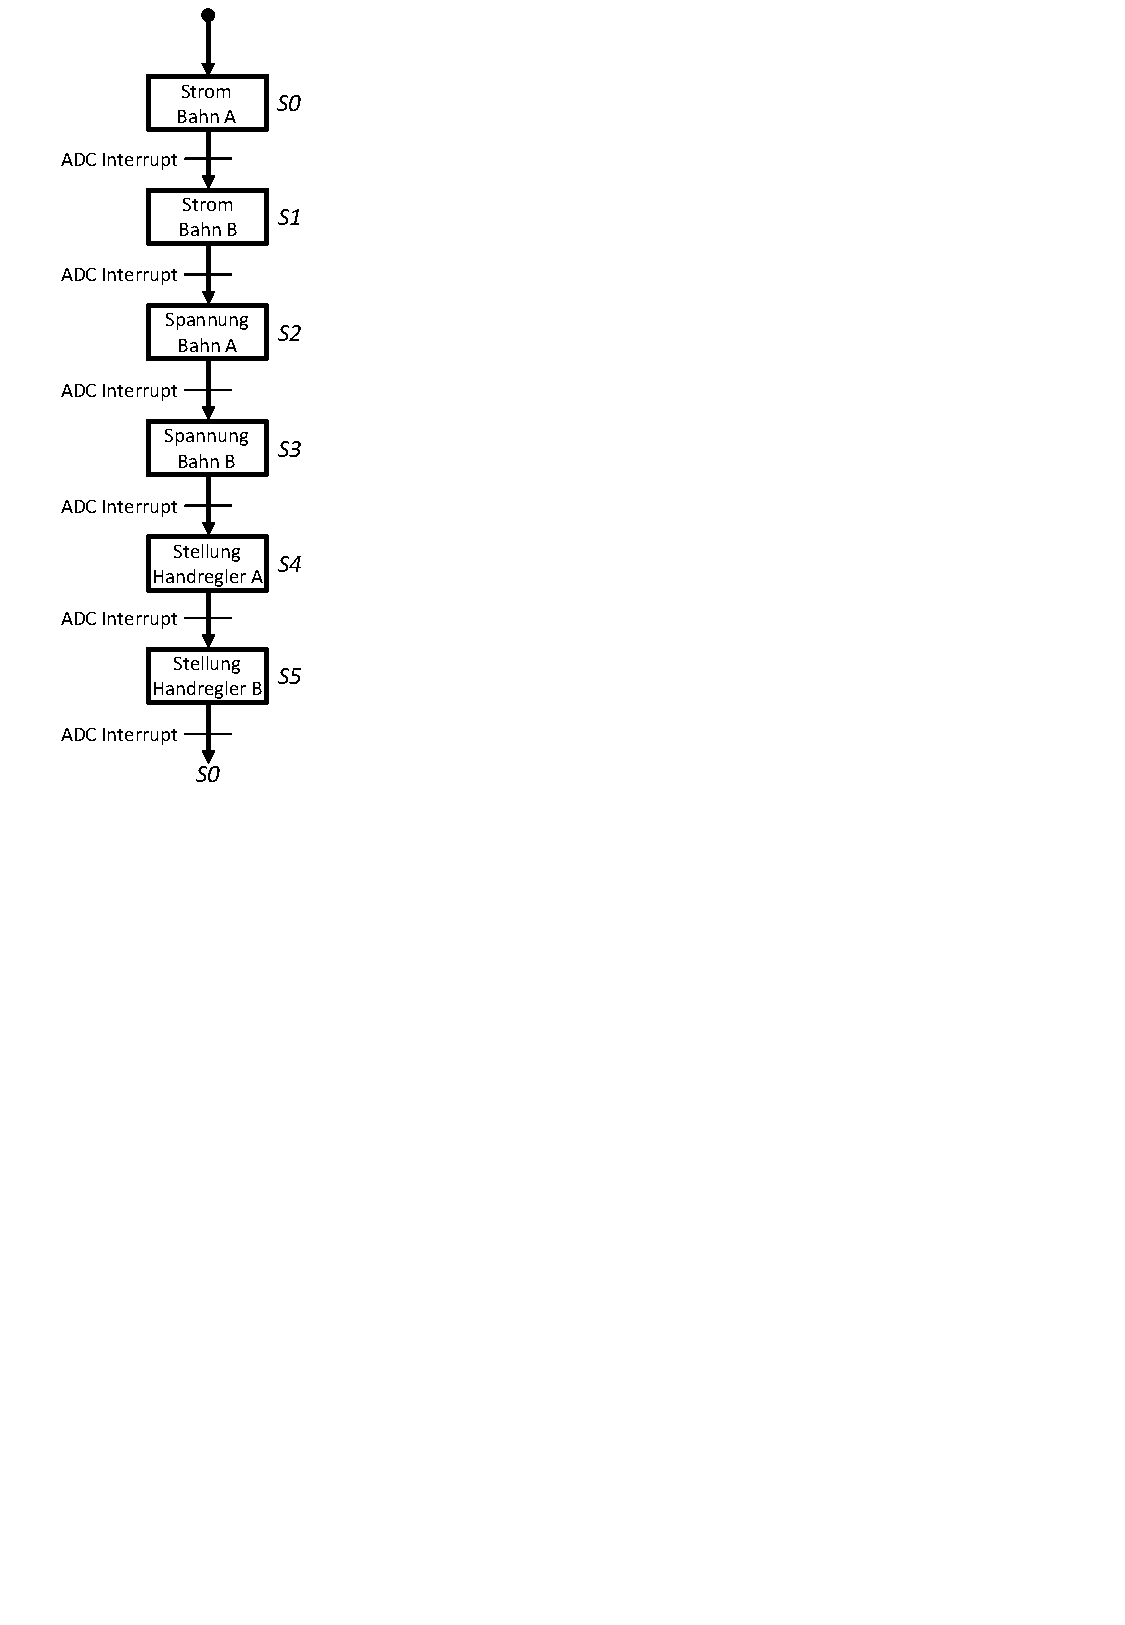
\includegraphics[width=0.3\textwidth]{rec/ADCAutomat.pdf}
			\caption[Zustandsautomat des MUX im ADC]{Zustandsautomat des MUX im ADC.\\Die Zustände(S0 bis S1) beschreiben, welcher ADC Pin des Mikrocontrollers gerade durch den MUX mit dem ADC verbunden ist. Die Transitionsbedingung (links) beschreibt das Ereignis, mit dem man von einem Zustand in den Nächsten wechselt. Ein Punkt markiert den Schritt in den Initialzustand (S0) des Automats und ein Pfeil einen Sprung zu einem darunter definierten Zustand.}
			\label{img:ADCMUX}
		\end{figure}

\subsection{PWM Generierung Tiefsetzsteller}\label{subsec:PWM}


\begin{figure}[htp]
	\centering
	\subcaptionbox{Zustandsautomat PWM Generierung
        \label{fig:PWMGENAut}}
        {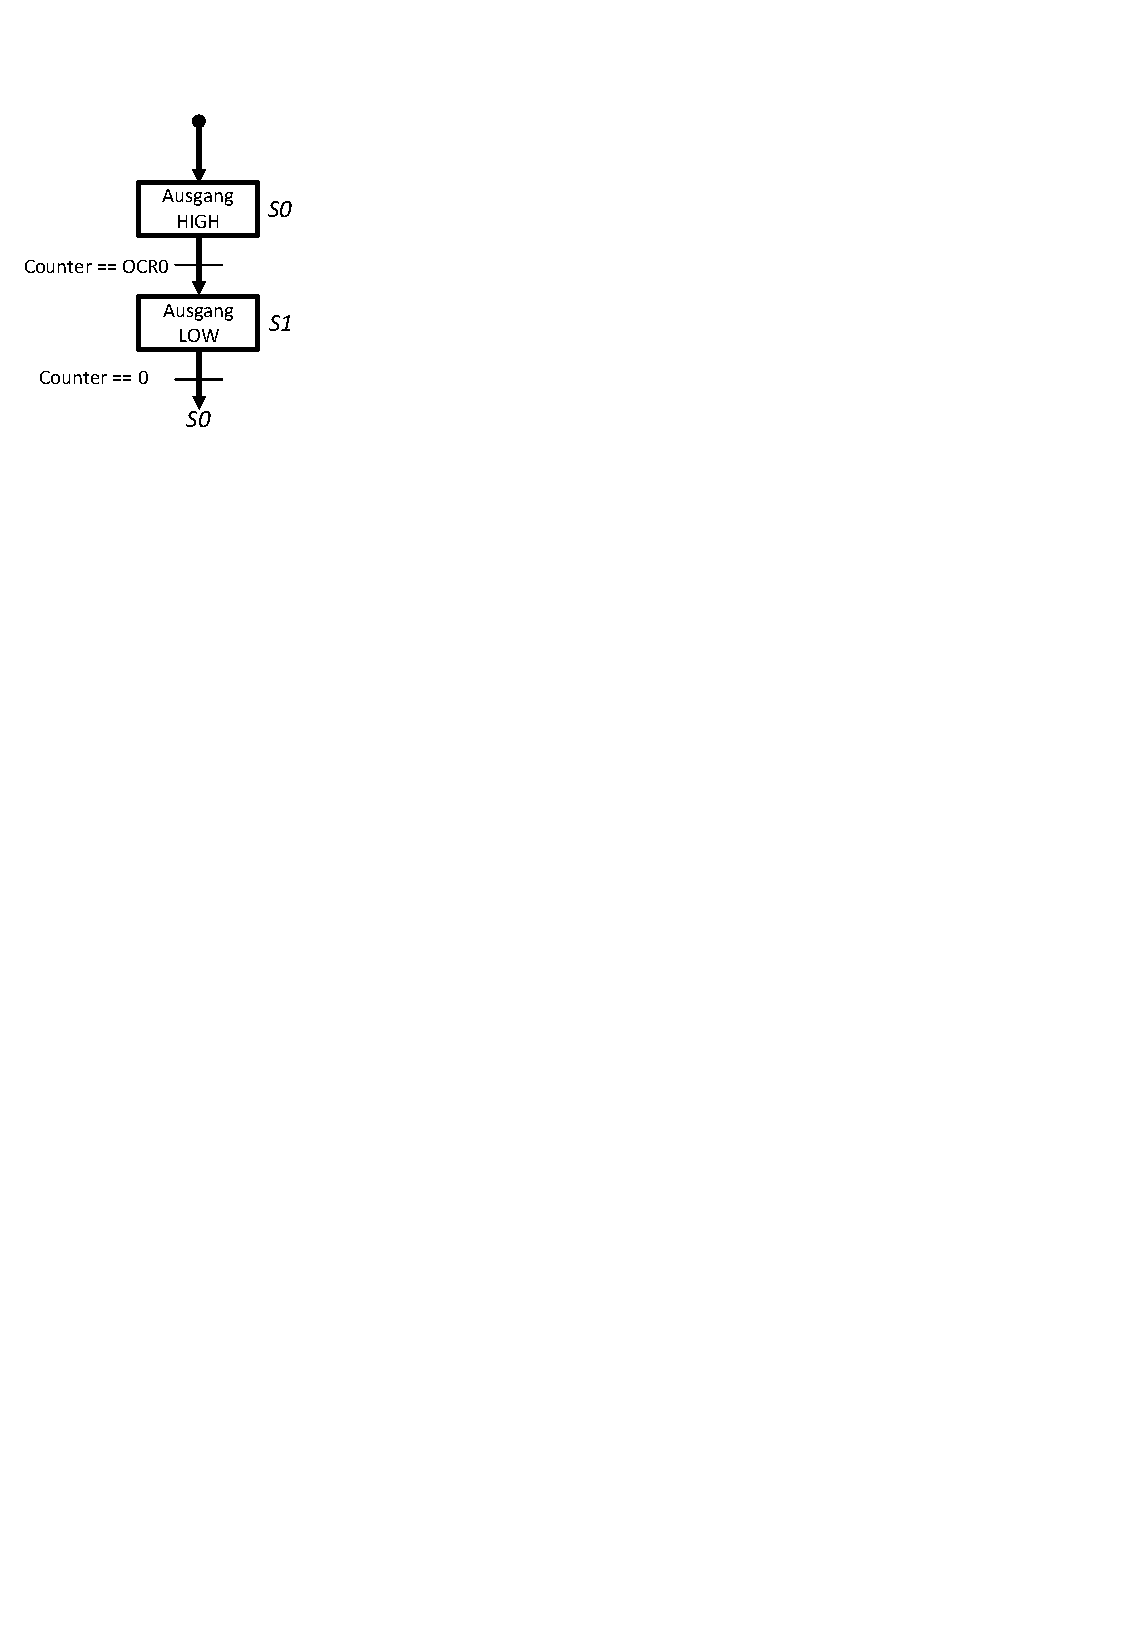
\includegraphics[width=0.34\textwidth]{rec/zustandsautomatPWM.pdf}}
        \hfill
  \subcaptionbox{Ausgang PWM Pin als Funktion des Zählerstands
        \label{fig:PWMGENFX}}
        {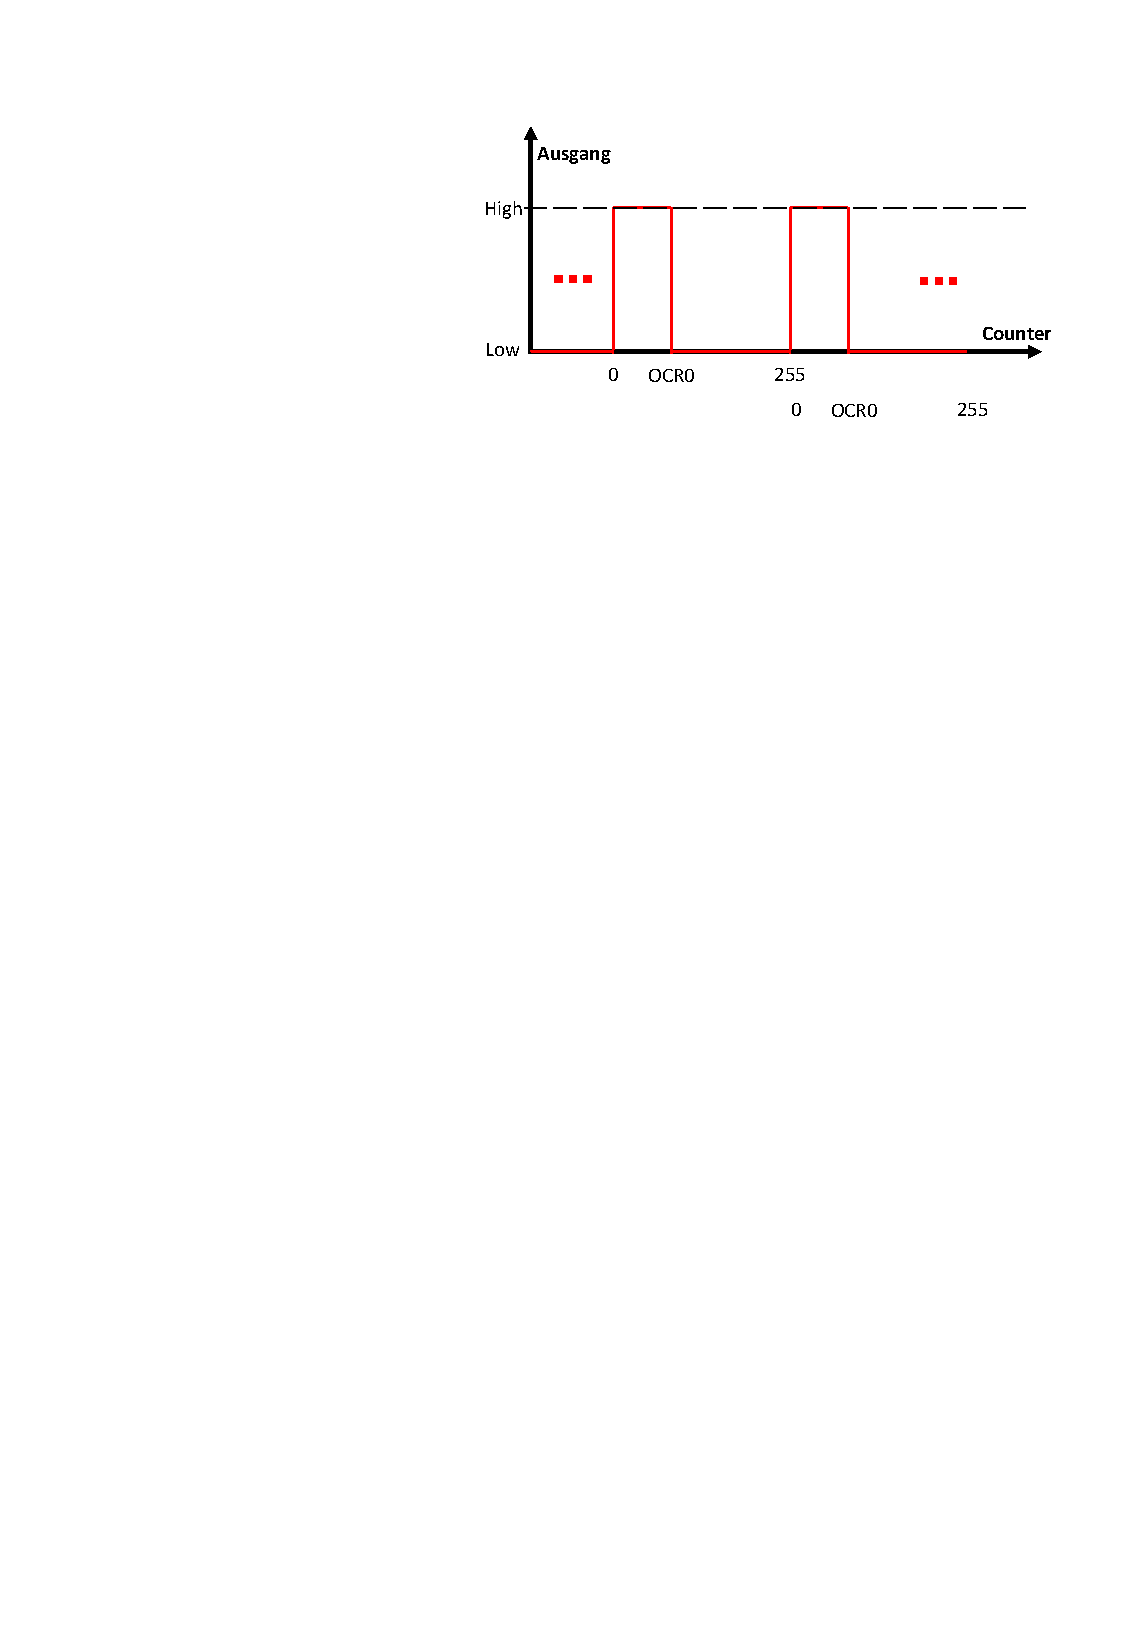
\includegraphics[width=0.64\textwidth]{rec/graphPWM.pdf}}
    \caption{Zustandsautomat des Timers zur PWM Generierung, sowie resultierendes Ausgangssignal bei konstantem Dutycycle.}


\end{figure}




Wie aus Abbildung \ref{fig:PWMGENFX} hervorgeht, ist das PWM Signal direkt eine Funktion des aktuellen Zählerstands von Timer0, sowie dem Inhalt des jeweiligen Overflow Compare Registers OCR0A/B.
Die PWM Generierung ist durch den Mikrocontroller in Hardware implementiert und muss lediglich aktiviert werden. Die Konfiguration dieser PWM Generierung ist in der Funktion initTimer implementiert und wird einmal zu Programmstart aufgerufen. Der Hardwaretimer setzt nun den jeweiligen Pin beim Überlauf des 8-bit Timers (Wert 0) auf High-Pegel und beim Erreichen des Wertes im OCR0AB Registers ( zum Beispiel  bei DutyCycle = 50\% OCR0A = 127 ) auf Low-Pegel.
Dieses Verhalten des Hardwaretimers ist zur Veranschaulichung nochmal in Abbildung  \ref{fig:PWMGENAut} als Zustandsautomat dargestellt.


\chapter{Bekannte Störungen}\label {cha:err}
Gelegentlich fallen Autos im Looping herunter.
Durch längere Tests und Analyse der Fehlerbilder, hat sich herausgestellt, dass dies kein Problem der Regelung selbst darstellt, sondern vielmehr der schlechten Qualität der zugekauften Carrera Bahn.
Genauer ist die Stromschiene der Bahn im Looping ein wenig in der Fahrbahnoberfläche versenkt und der Übergang zwischen den zusammengesteckten Streckenstücken weist einen unstetigen Verlauf auf. Dadurch ergibt sich eine Diskontinuität des Stroms, durch den Antrieb des Fahrzeugs im Looping. Dies führt zu Geschwindigkeitsverlust , sowie letztendlich zum Absturz des Fahrzeugs. Werden nun, um die schlechte mechanische Beschaffenheit auszugleichen,  die Strombürsten des Fahrzeugs weiter in Richtung Schiene gebogen, taucht die Führungsnase nicht mehr weit genug in die Bahn ein und das Fahrzeug fliegt aus der Kurve oder triggert die Sensoren nicht mehr verlässlich.

\chapter{Bedienungsanleitung}
%evt bild von visu
\section{Einschalten}
	Die Anlage muss zum Einschalten lediglich mit der Netzversorgung verbunden werden. Sobald die Anlage Spannung hat, bootet der RaspberryPi selbständig und startet die Visualisierung. Ab diesem Punkt ist die Carrera Bahn betriebsbereit und im Modus manuelles Fahren (Abschnitt \ref{subsec:ManuellesFahren}).
\section{Betrieb}
	\begin{figure}[ht]
		\centering
		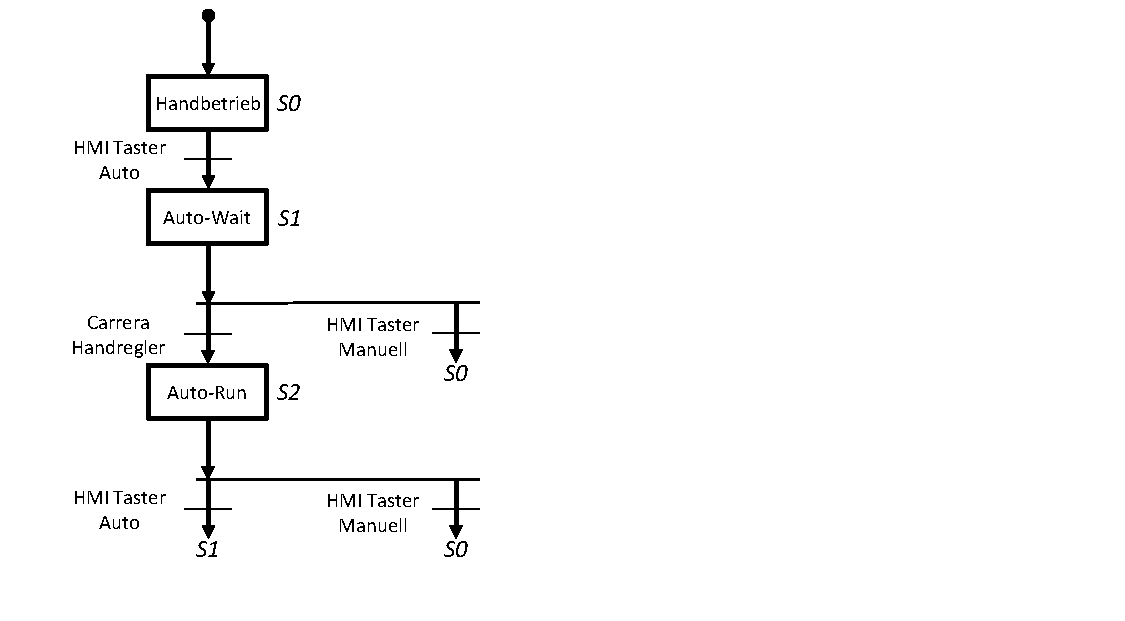
\includegraphics[width=0.5\textwidth]{rec/modiAuswahl.pdf}
		\caption[Zustandsautomat zum Wechsel der Betriebsmodi einer Bahn]{Zustandsautomat zum Wechsel der Betriebsmodi einer Bahn.\\Durch den \glqq HMI Taster Auto\grqq{} der jeweiligen Bahn, kann der Nutzer immer in den \glqq Auto-Wait\grqq{} Zustand (S1) wechseln, in dem das Auto hält. Von diesem Zustand aus, kann der Nutzer die Bahn durch Betätigung des Handreglers, in den \glqq Auto-Run\grqq Zustand{} (S2) versetzten und das Auto fährt anschließend selbständig. Aus jedem Zustand kann der Nutzer mit dem \glqq HMI Taster Manuell\grqq{}, die Bahn in den manuellen Modus versetzten und das entsprechende Auto mit dem Handregler konventionell steuern.}
		\label{img:Betriebsmodi}
	\end{figure}
	Die Carrera Bahn beherrscht 2 Modi.
	\begin{itemize}
		\item Manuelles Fahren
		\item Automatisiertes Fahren
	\end{itemize}
	Die Modi können unabhängig voneinander auf beiden Bahnen gewählt werden, sodass es zum Beispiel möglich ist, manuell gegen ein automatisiertes Fahrzeug anzutreten. Die Wahl eines dementsprechenden Modus (automatisiert oder manuell), wird durch eine LED über, beziehungsweise unter, des jeweiligen Tasters des gewählten Modus signalisiert. Außerdem kann die Energieversorgung jeder Bahn mit dem entsprechenden Wechselschalter ausgewählt werden. Unabhängig des gewählten Modus, wird in der Visualisierung die Zeit der zwei Streckenabschnitte, sowie die Rundenzeit angezeigt.
In der Visualisierung ist die Strecke von der Startlinie bis vor den Looping in Streckenabschnitt 1 zusammengefasst.
			Der Rest einer Runde (vor dem Looping bis zur Startlinie) bildet Streckenabschnitt 2.
Nach 30 Runden ist das Rennen vorbei und die Visualisierung wird statisch.
	Der Wechsel zwischen den Modi findet nach Abbildung \ref{img:Betriebsmodi} statt und ist in den jeweiligen Abschnitten genauer erklärt.
	\subsection{Manuelles Fahren}\label{subsec:ManuellesFahren}
		Im Modus Manuelles Fahren kann das Fahrzeug konventionell, über die originalen Carrera Handregler, gesteuert werden. Durch Betätigung des HMI-Tasters Auto, kann die Bahn in den Auto-Wait Zustand versetzt werden. 
\newpage
	\subsection{Automatisiertes Fahren}\label{subsec:bedAuto}
		Der automatisierte Modus ist aufgeschlüsselt in zwei Zustände:
		\begin{itemize}
			\item Auto-Wait
			\item Auto-Run
		\end{itemize}
		\subsubsection{Auto-Wait}
		Immer wenn in den Modus des automatisierten Fahrens gewechselt wird, startet die Steuerung in
		Auto-Wait und das Auto steht.
		Durch kurzes durchdrücken des zugehörigen Handreglers, wechselt das Auto in den Auto-Run Zustand.
		\subsubsection{Auto-Run}
			Im Auto-Run Zustand fährt das Auto selbständig. Durch die Regelung der Geschwindigkeit des langsamen Streckenabschnitts, 
			braucht das Auto einige Runden um die optimale Spannung, für diese Geschwindigkeit zu finden. Dies ist genauer in Abschnitt \ref{subsubsec:Tcontrol} beschrieben.
			Es ist darauf zu achten, dass wenn das Auto im Looping herunterfällt, es wieder an der Startlinie eingesetzt wird. Ist dies nicht der Fall, 
			ist weiterhin die erhöhte Geschwindigkeit aus dem Looping aktiv und das Auto verlässt in der nächsten Kurve erneut die Bahn. 
\section{Ausschalten}
Um die Anlage ordnungsgemäß herunterzufahren, ist der Reset Taster am HMI (Abbildung \ref{img:hid} - Reset Visualisierung) mindestens fünf Sekunden gedrückt zu halten.
Nun muss der Nutzer warten bis der RaspberryPi komplett heruntergefahren ist. Dies ist daran zu erkennen, dass die grüne LED auf dem RaspberryPi nicht mehr blinkt und der Bildschirm in den Standby-Modus schaltet.
\chapter{Reflexion}

Die zu Beginn, in Abschnitt \ref{sec:ziel} definierten Probleme der vorhandenen Carrera Bahn, sind durch das neue Steuer-/Regelkonzept, sowie eine neue Hardware Architektur, fast alle beseitigt.\\
Da nun unabhängig der gewählten Energiequelle, die Bahnspannung immer durch die Tiefsetzsteller erzeugt und geregelt wird, ist diese nicht mehr von der eigentlichen Quelle abhängig.
Somit stellt nun auch die Solarenergieversorgung eine stabilisierte Spannungsquelle dar (siehe Abschnitt \ref{subsubsec:Ucontrol}).\\
Der Temperaturdrift, des in der vorherigen Bahn eingesetzten variablen Widerstands, ist behoben, da dieser in der neuen Anlage, durch die Möglichkeit die Bahnspannung durch den Dutycycle der Tiefsetzsteller anzupassen, nicht mehr benötigt wird. (siehe Abbildung \ref{img:energiefluss})\\
Die Framerate der Visualisierung wurde angehoben, indem immer nur der dynamische Bildinhalt (die Rundenzeiten) neu gerendert wird (siehe Abschnitt \ref{sec:SoftPi}). Dies reduziert die Rechenzeit pro Frame.\\
Die Probleme mit Aliasing beim Auslesen der Sensoren sind durch den Einsatz der \glqq Pin Change Interrupts\grqq{} des Arduinos zum Digitalisieren der Sensorsignale vollständig behoben (siehe Abschnitt \ref{subsubsec:PCINT}).\\

Ein bestehendes Problem der Carrera Bahn ist, das gelegentlich ein Auto im Looping herunterfällt, wenn dieses automatisch fährt. Die Ursache dessen wurde identifiziert (siehe Abschnitt \ref{cha:err}), kann allerdings nicht mit vertretbarem Aufwand gelöst werden.

Insgesamt wird die Projektarbeit vom Autor als Erfolg angesehen.
\chapter{Quellenverzeichnis}
Scout1. (September 2004). Interrupt Programme.gif – Mikrocontroller.net.
\\Von Mikrocontroller.net: \href{https://www.mikrocontroller.net/articles/Datei:Interrupt_Programme.gif}
{\url{https://www.mikrocontroller.net/articles/Datei:Interrupt_Programme.gif}} abgerufen \label{src:scout1}
\chapter{Anhang}


	\begin{table}[H]
	\centering
		\caption{Pinbelegung der Sub-D Buchse auf dem HMI}
		\begin{tabular}{|l|l|}
			\hline
			\textbf{Sub-D Pin} &\textbf{Funktion}\\
			\hline
			\hline
			1 & VCC (5V)\\
			\hline
			2 & GND\\
			\hline
			3 & -\\
			\hline
			4 & -\\
			\hline
			5 & -\\
			\hline
			6 & Sensor 0\\
			\hline
			7 & Sensor 1\\
			\hline
			8 & Sensor 2\\
			\hline
			9 & Sensor 3\\
			\hline
			10 & Sensor 4\\
			\hline
			11 & Sensor 5\\
			\hline
			12 & Schiene A - Plus\\
			\hline
			13 & Schiene A - Minus\\
			\hline
			14 & Schiene B - Plus\\
			\hline
			15 & Schiene B - Minus\\
			\hline
		\end{tabular}
		\label{tab:AnhangBelegungSUBD}
	\end{table}

	\begin{table}[H]
	\centering
		\caption{Pinbelegung GPIO RaspberryPi}
		\begin{tabular}{|l|l|}
			\hline
			\textbf{Raspberry Pin} &\textbf{Funktion}\\
			\hline
			\hline
			1 & VCC MCU (3V3)\\
			\hline
			2 & VCC Input (5V)\\
			\hline
			3$\rightarrow$5 & -\\
			\hline
			6 & GND Input\\
			\hline
			7 & -\\
			\hline
			8 & -\\
			\hline
			9 & -\\
			\hline
			10 & RXD UART\\
			\hline
			11$\rightarrow$40 & -\\
			\hline
		\end{tabular}
		
		\label{tab:AnhangBelegungRPI}
	\end{table}

	\begin{table}[hb]
		\caption{Pinbelegung des Arduino}
		\begin{tabular}{|l|l|l|}
			\hline
			\textbf{Arduino Pin} & \textbf{Atmel Pin} &\textbf{Funktion}\\
			\hline
			\hline
			0 &  & Ohne Funktion\\
			\hline
			1 &  & Ohne Funktion\\
			\hline
			2 &  & Ohne Funktion\\
			\hline
			3 &  & Ohne Funktion\\
			\hline
			4 & OC0B & PWM Tiefsetzsteller Schiene B\\
			\hline
			5 &  & Ohne Funktion\\
			\hline
			6 &  & Ohne Funktion\\
			\hline
			7 &  & Ohne Funktion\\
			\hline
			8 &  & Ohne Funktion\\
			\hline
			9 &  & Ohne Funktion\\
			\hline
			10 & PCINT4 & Taster HID \glqq Schiene B - Automatik\grqq \\
			\hline
			11 & PCINT5 & Taster HID \glqq Schiene B - Manuell\grqq \\
			\hline
			12 & PCINT6 & Taster HID \glqq Schiene A - Automatik\grqq \\
			\hline
			13 &  OC0A & PWM Tiefsetzsteller Schiene A\\
			\hline
			14	& PCINT10	& Taster HID \\
				&		& \glqq Schiene B - Reset Regler Bahngeschwindigkeit\grqq \\
			\hline
			15 	& PCINT9 	& Taster HID \\
				&		& \glqq Schiene A - Reset Regler Bahngeschwindigkeit\grqq \\
			\hline
			16 &  & Ohne Funktion\\
			\hline
			17 &  & Ohne Funktion\\
			\hline
			18 &  & Serielle Verbindung zu RaspberryPi\\
			\hline
			19$\rightarrow$45 &  & Ohne Funktion\\
			\hline
			46 & PL3 & HID LED \glqq Schiene B - Manuell\\
			\hline
			47 & PL2 & HID LED \glqq Schiene B - Automatik\\
			\hline
			48 & PL1 & HID LED \glqq Schiene A - Manuell\\
			\hline
			49 & PL0 & HID LED \glqq Schiene A - Automatik\\
			\hline
			A1$\rightarrow$A0 & ADC1$\rightarrow$ADC0 & Shunt Tiefsetzsteller Schiene A\\
			\hline
			A3$\rightarrow$A2 & ADC3$\rightarrow$ADC2 & Shunt Tiefsetzsteller Schiene B\\
			\hline
			A4 & ADC4 & Spannung Schiene A\\
			\hline
			A5 & ADC5 & Spannung Schiene B\\
			\hline
			A6 & ADC6 & Carrera Handregler Schiene A\\
			\hline
			A7 & ADC7 & Carrera Handregler Schiene B\\
			\hline
			A8 & PCINT16 & Sensor 0 (Schiene A - Startlinie)\\
			\hline
			A9 & PCINT17 & Sensor 1 (Schiene A - vor dem Looping)\\
			\hline
			A10 & PCINT18 & Sensor 2 (Schiene A - nach dem Looping)\\
			\hline
			A11 & PCINT19 & Sensor 3 (Schiene B - Startlinie)\\
			\hline
			A12 & PCINT20 & Sensor 4 (Schiene B - vor dem Looping)\\
			\hline
			A13 & PCINT21 & Sensor 5 (Schiene B - nach dem Looping)\\
			\hline
			A14 & PCINT22 & Taster HID \glqq Reset Rundenzeit Visualisierung\grqq \\
			\hline
			A15 & PCINT23 & Taster HID \glqq Schiene A - Manuell\grqq \\
			\hline
		\end{tabular}
		
		\label{tab:AnhangBelegungArduino}
	\end{table}

	\clearpage
	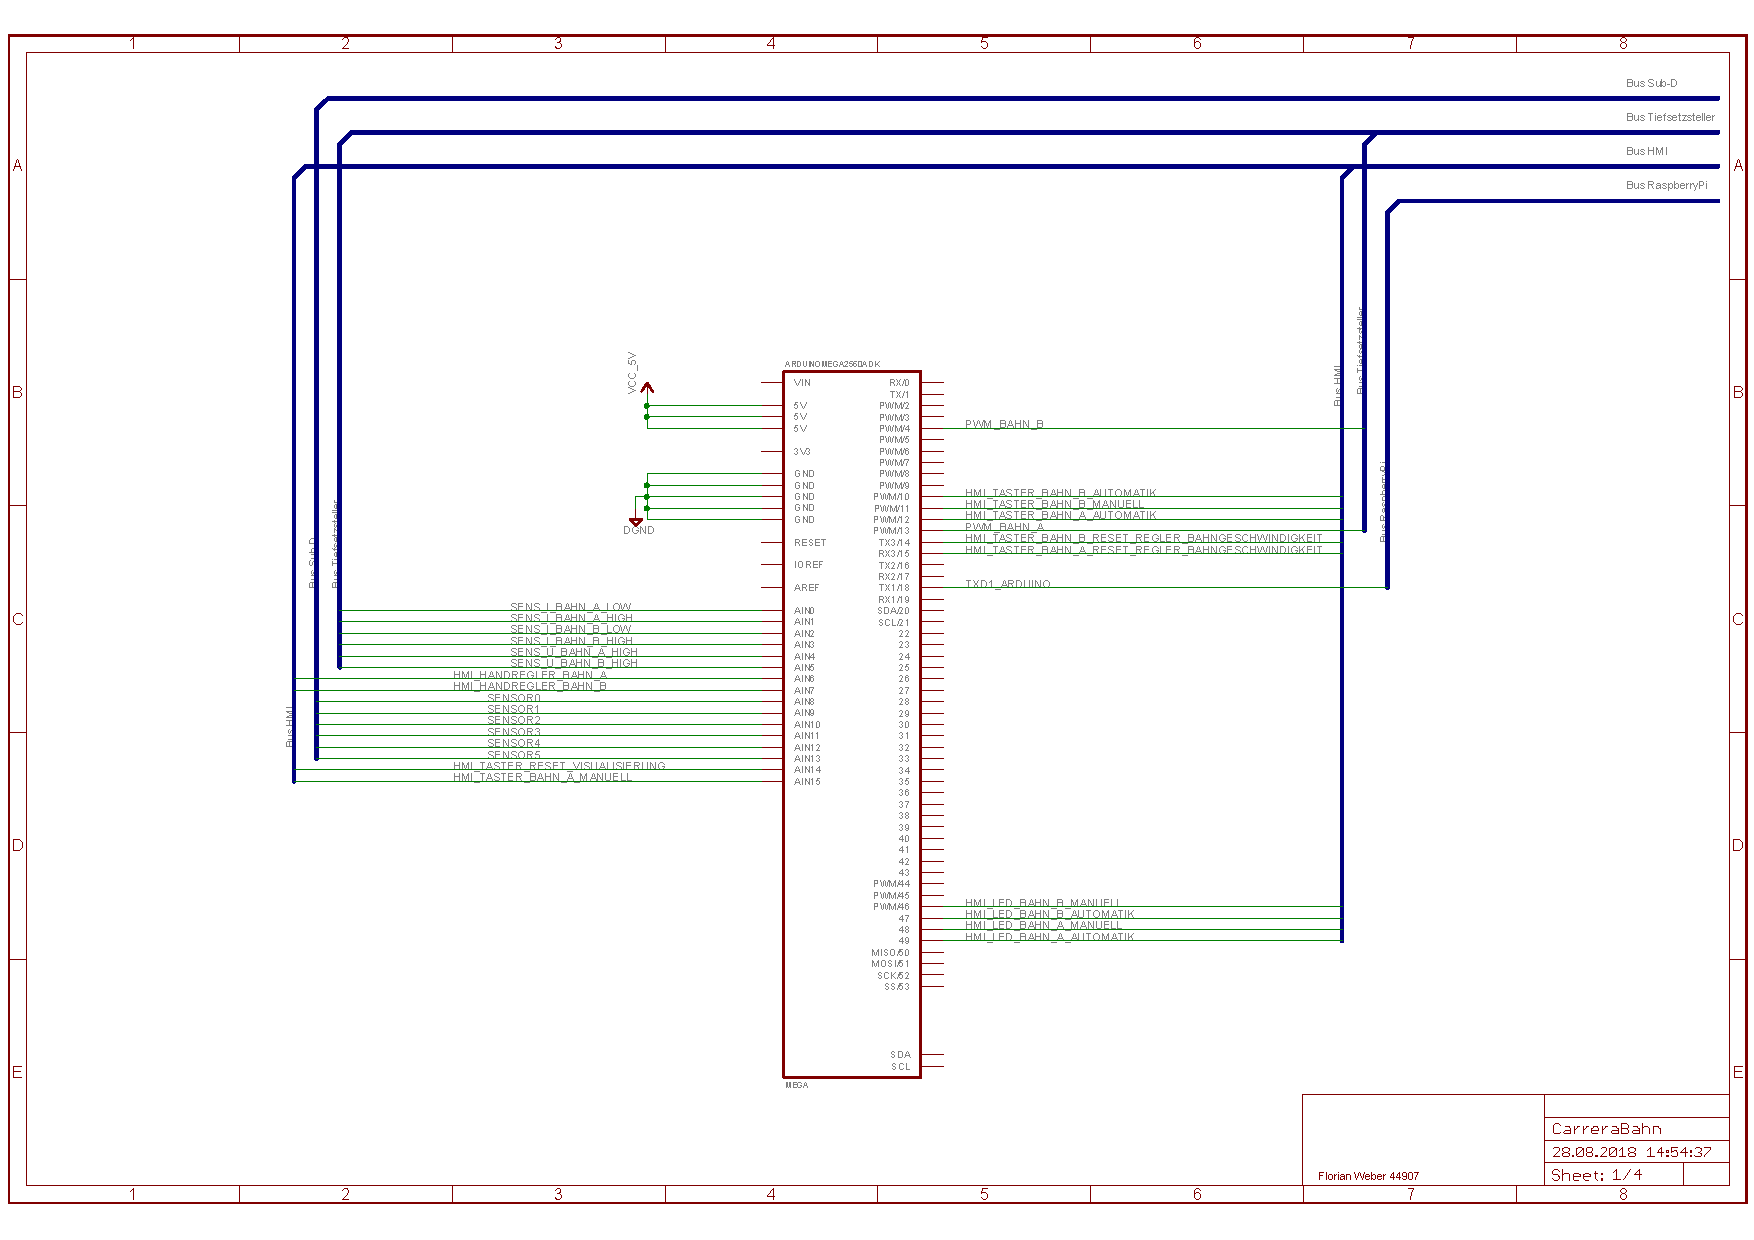
\includepdf[pages=-,landscape=true,trim=0cm 0cm 0cm 0cm,clip]{rec/schematic/CarreraBahn.pdf}
	%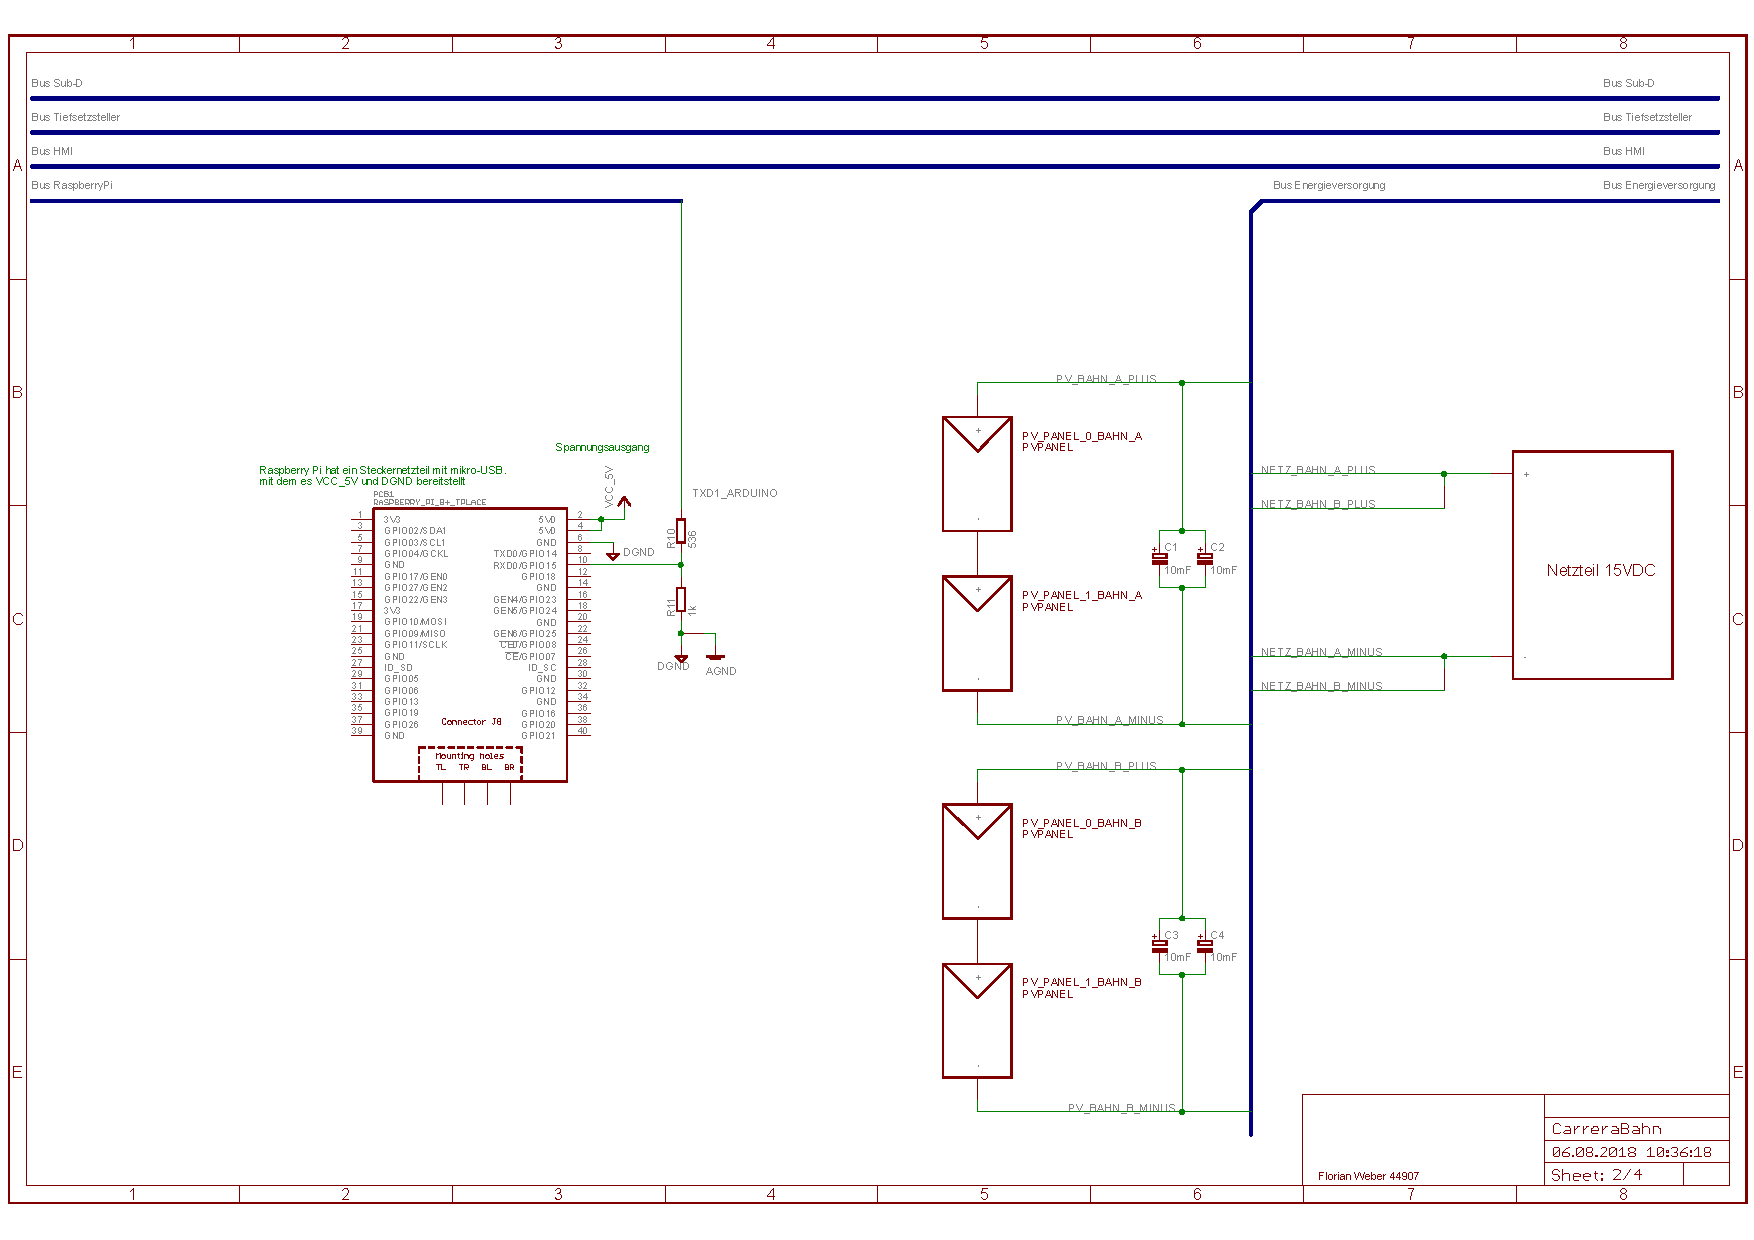
\includepdf[landscape=true,trim=0cm 0cm 0cm 0cm,clip]{rec/schematic/2.pdf}
	%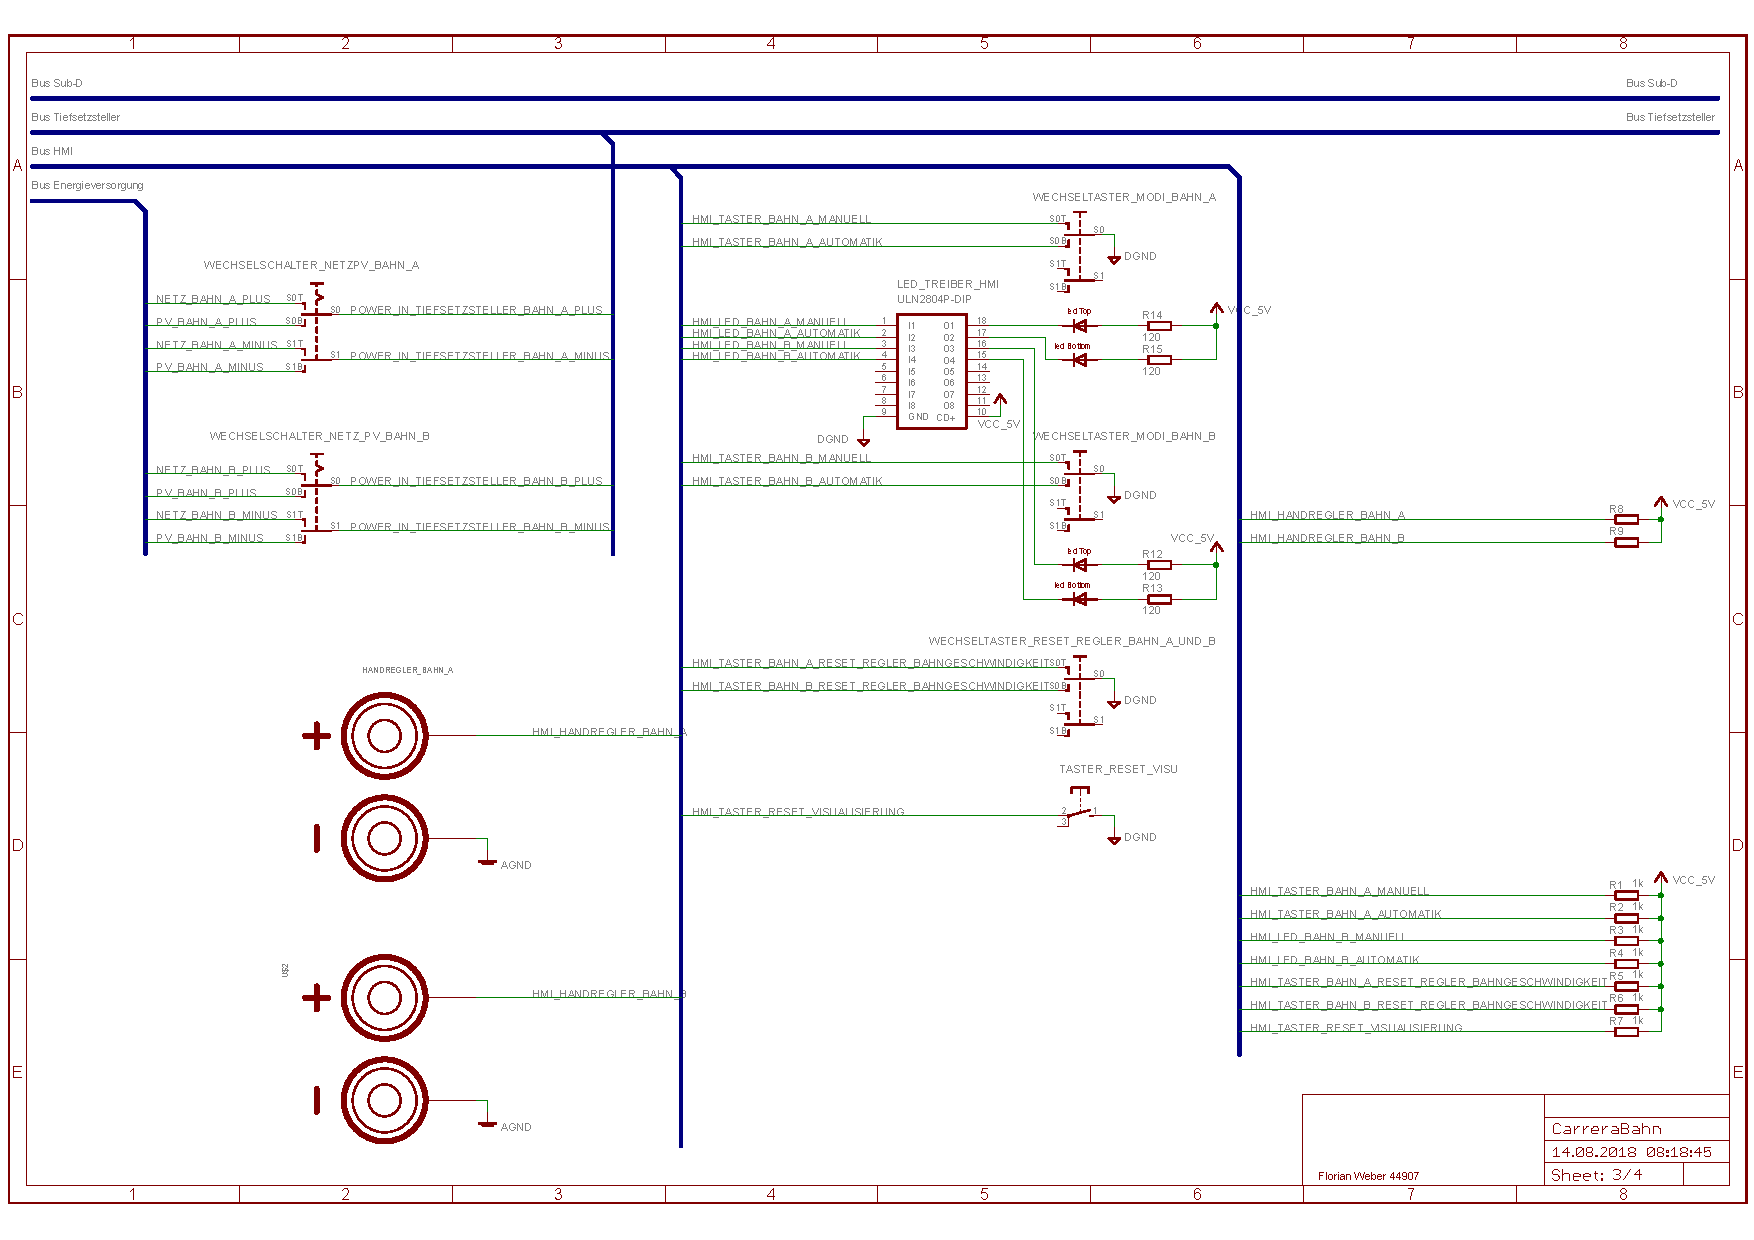
\includepdf[landscape=true,trim=0cm 0cm 0cm 0cm,clip]{rec/schematic/3.pdf}
	%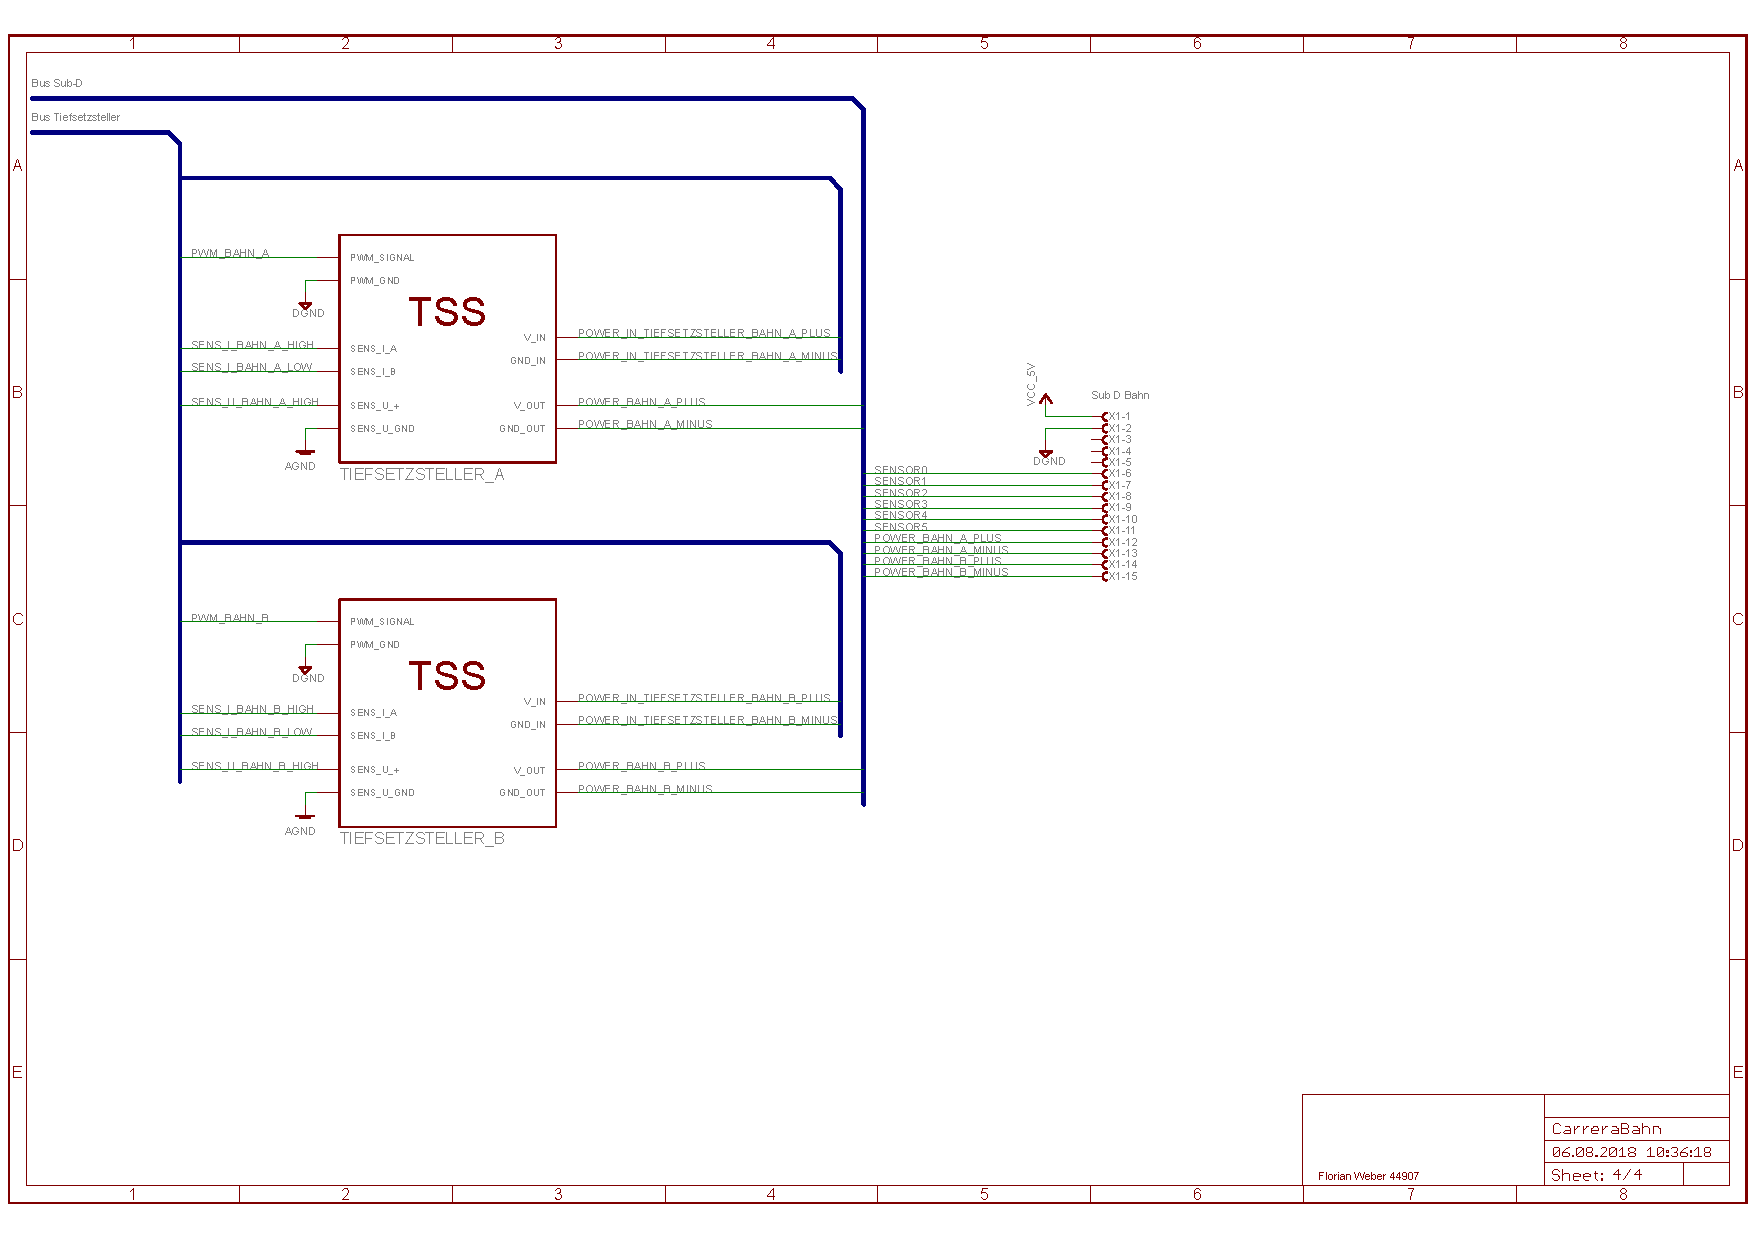
\includepdf[landscape=true,trim=0cm 0cm 0cm 0cm,clip]{rec/schematic/4.pdf}

\end{document}
